\section{Results}
\label{sec:results}

\subsection{Summary}

\begin{table}[H]
\centering\small
\caption{Best $(a,b,s)$ of the \Ks{} fit per run period and mass version (the joint \Ks+\La{} fit gives the same point where
the last column says ``yes''), \Ks{} Baker--Cousins $\chi^2$/ndf, and the \La{} $\chi^2$ at the \Ks{} best point minus the \La{}
minimum ($\Delta\chi^2_\Lambda$). Uncertainties and the \La-only and joint fits: Table~\ref{tab:fits}.}
\label{tab:summary}
\begin{tabular}{llcccccc}
\toprule
period & mass & $a$ (\%/(GeV/$c$)) & $b$ (\%) & $s$ & $\chi^2_{K}$/ndf & $\Delta\chi^2_\Lambda$ & joint = \Ks \\
\midrule
% generated by scripts/make_numbers.py
A & KFP mass & 3.00 & 1.60 & 0.991 & 470.4/389 & 2.2 & yes \\
 & recomputed, no $\kappa$ & 3.00 & 1.60 & 0.991 & 464.5/389 & 3.4 & yes \\
 & recomputed, with $\kappa$ & 1.50 & 1.40 & 0.999 & 468.5/389 & 6.1 & yes \\
\midrule
B & KFP mass & 4.00 & 1.20 & 0.991 & 400.5/389 & 13.8 & no \\
 & recomputed, no $\kappa$ & 4.00 & 1.20 & 0.991 & 473.1/389 & 30.5 & yes \\
 & recomputed, with $\kappa$ & 2.00 & 1.40 & 0.998 & 457.4/389 & 4.8 & yes \\
\midrule
all & KFP mass & 3.75 & 1.40 & 0.991 & 421.5/389 & 13.9 & yes \\
 & recomputed, no $\kappa$ & 3.50 & 1.40 & 0.991 & 462.1/389 & 25.0 & yes \\
 & recomputed, with $\kappa$ & 1.75 & 1.40 & 0.998 & 473.9/389 & 9.0 & no \\

\bottomrule
\end{tabular}
\end{table}

\paragraph{Effect of the correction} (``no $\kappa$'' $\to$ ``with $\kappa$'', same candidates):
\begin{itemize}
\item \textbf{Scale.} $s=\PerARawKsS\to\PerAKapKsS$ (A) and $\PerBRawKsS\to\PerBKapKsS$ (B). The \La-only fits agree with
  $\kappa$ ($s=\PerAKapLaS$ and \PerBKapLaS). The \pt-integrated \Ks{} Gaussian peak moves from
  $\PerARawKsGM\pm\PerARawKsGMe$ to $\PerAKapKsGM\pm\PerAKapKsGMe$\mevcc{} (A; $\PerARawKsGPull\sigma$ and
  $\PerAKapKsGPull\sigma$ from PDG) and from $\PerBRawKsGM\pm\PerBRawKsGMe$ to $\PerBKapKsGM\pm\PerBKapKsGMe$\mevcc{} (B;
  $\PerBRawKsGPull\sigma$, $\PerBKapKsGPull\sigma$). With $\kappa$ the \Ks{} peak is still \PerAKapKsBelow{} (A) and \PerBKapKsBelow\mevcc{} (B) below PDG; the fitted
  $s<1$ reflects the same residual.
\item \textbf{Resolution.} $a$ is reduced to \PerAARatio{} (A) and \PerBARatio{} (B) of its value without $\kappa$; $b$ changes from
  \PerARawKsB{} to \PerAKapKsB\% (A) and from \PerBRawKsB{} to \PerBKapKsB\% (B). The \Ks{} Gaussian width at V0 $\pt=1.6$--2.2\gevc{} drops from \PerARawKsWidHigh{} to
  \PerAKapKsWidHigh\mevcc{} (A) and from \PerBRawKsWidHigh{} to \PerBKapKsWidHigh\mevcc{} (B) (Table~\ref{tab:peaksks}).
  Interpretation: without the correction the charge-odd and $\varphi$/$\eta$-dependent scale distortion that $\kappa$ removes
  broadens the mass peak ($\pi^+$ and $\pi^-$ are shifted in opposite directions, more at high \pt), and the fit absorbs this into
  $a$. This interpretation is not tested separately.
\item \textbf{\Ks/\La{} consistency.} $\Delta\chi^2_\Lambda$ = \PerARawDchiLa{} $\to$ \PerAKapDchiLa{} (A) and \PerBRawDchiLa{}
  $\to$ \PerBKapDchiLa{} (B). The \Ks/\La{} difference stays small in period A and largely disappears in period B with the correction.
\item \textbf{Periods.} After the correction period B still has a larger curvature term than period A
  ($a=\PerBKapKsA^{+\PerBKapKsAUp}_{-\PerBKapKsADn}$ vs $\PerAKapKsA^{+\PerAKapKsAUp}_{-\PerAKapKsADn}$\%/(GeV/$c$)), as it had
  before (Sec.~\ref{sec:rundep}).
\item \textbf{Fit quality.} With $\kappa$ the \Ks{} $\chi^2$ is \PerAKapKsChi/\PerAKapKsNdf{} (A) and \PerBKapKsChi/\PerBKapKsNdf{}
  (B), against \PerARawKsChi{} and \PerBRawKsChi{} without. In period B the KFP-mass fit has a clearly lower $\chi^2$
  (\PerBKfpKsChi) than both recomputed versions (KFP best point $a=\PerBKfpKsA$\%/(GeV/$c$), $b=\PerBKfpKsB$\%, $s=\PerBKfpKsS$; open issue).
\end{itemize}

\begin{table}[H]
\centering\footnotesize
\caption{All fits: \Ks, \La+$\bar\Lambda$ and joint, per period and mass version. Profile $\Delta\chi^2=1$ intervals on
the grid (statistical only); $\Delta\chi^2_\Lambda$ as in Table~\ref{tab:summary}; ``edge'' = best point on the grid boundary.
From \fpath{logs/fitMomRes_k287_<period>_<version>.txt}.}
\label{tab:fits}
\setlength{\tabcolsep}{4pt}
\begin{tabular}{lllcccccc}
\toprule
 & mass & fit & $a$ (\%/(GeV/$c$)) & $b$ (\%) & $s$ & $\chi^2$/ndf & $\Delta\chi^2_\Lambda$ & edge \\
\midrule
% generated by scripts/make_numbers.py
A & KFP mass & \Ks & $3.00^{+0.06}_{-0.27}$ & $1.60^{+0.03}_{-0.05}$ & $0.9910^{+0.0001}_{-0.0001}$ & 470.4/389 & 2.2 & no \\
 &  & \La & $1.75^{+0.72}_{-1.75}$ & $2.00^{+0.37}_{-0.83}$ & $0.9900^{+0.0040}_{-0.0017}$ & 261.8/247 &  & no \\
 &  & joint & $3.00^{+0.06}_{-0.27}$ & $1.60^{+0.03}_{-0.03}$ & $0.9910^{+0.0001}_{-0.0001}$ & 734.5/639 &  & no \\
\addlinespace
A & recomputed, no $\kappa$ & \Ks & $3.00^{+0.12}_{-0.13}$ & $1.60^{+0.01}_{-0.10}$ & $0.9910^{+0.0002}_{-0.0001}$ & 464.5/389 & 3.4 & no \\
 &  & \La & $4.25^{+0.30}_{-0.18}$ & $1.60^{+0.10}_{-0.22}$ & $0.9910^{+0.0007}_{-0.0009}$ & 293.2/247 &  & no \\
 &  & joint & $3.00^{+0.05}_{-0.08}$ & $1.60^{+0.02}_{-0.04}$ & $0.9910^{+0.0002}_{-0.0001}$ & 761.1/639 &  & no \\
\addlinespace
A & recomputed, with $\kappa$ & \Ks & $1.50^{+0.02}_{-0.16}$ & $1.40^{+0.01}_{-0.01}$ & $0.9990^{+0.0000}_{-0.0001}$ & 468.5/389 & 6.1 & no \\
 &  & \La & $3.25^{+0.60}_{-0.45}$ & $1.20^{+0.08}_{-0.30}$ & $0.9980^{+0.0022}_{-0.0004}$ & 252.7/247 &  & no \\
 &  & joint & $1.50^{+0.02}_{-0.08}$ & $1.40^{+0.01}_{-0.01}$ & $0.9990^{+0.0000}_{-0.0001}$ & 727.3/639 &  & no \\
\midrule
B & KFP mass & \Ks & $4.00^{+0.29}_{-0.18}$ & $1.20^{+0.15}_{-0.05}$ & $0.9910^{+0.0001}_{-0.0008}$ & 400.5/389 & 13.8 & no \\
 &  & \La & $6.00^{+0.37}_{-0.28}$ & $1.80^{+0.18}_{-0.17}$ & $0.9970^{+0.0026}_{-0.0010}$ & 276.2/247 &  & no \\
 &  & joint & $4.00^{+0.34}_{-0.28}$ & $1.40^{+0.06}_{-0.23}$ & $0.9910^{+0.0001}_{-0.0007}$ & 689.1/639 &  & no \\
\addlinespace
B & recomputed, no $\kappa$ & \Ks & $4.00^{+0.05}_{-0.07}$ & $1.20^{+0.06}_{-0.04}$ & $0.9910^{+0.0001}_{-0.0002}$ & 473.1/389 & 30.5 & no \\
 &  & \La & $5.25^{+0.33}_{-0.29}$ & $3.00^{+0.10}_{-0.11}$ & $1.0050^{+0.0009}_{-0.0017}$ & 287.9/247 &  & no \\
 &  & joint & $4.00^{+0.05}_{-0.36}$ & $1.20^{+0.23}_{-0.02}$ & $0.9910^{+0.0001}_{-0.0002}$ & 791.5/639 &  & no \\
\addlinespace
B & recomputed, with $\kappa$ & \Ks & $2.00^{+0.05}_{-0.09}$ & $1.40^{+0.04}_{-0.02}$ & $0.9980^{+0.0002}_{-0.0000}$ & 457.4/389 & 4.8 & no \\
 &  & \La & $3.50^{+0.16}_{-0.72}$ & $1.40^{+0.24}_{-0.13}$ & $1.0010^{+0.0008}_{-0.0014}$ & 284.0/247 &  & no \\
 &  & joint & $2.00^{+0.06}_{-0.06}$ & $1.40^{+0.03}_{-0.02}$ & $0.9980^{+0.0002}_{-0.0000}$ & 746.2/639 &  & no \\
\midrule
all & KFP mass & \Ks & $3.75^{+0.07}_{-0.27}$ & $1.40^{+0.05}_{-0.05}$ & $0.9910^{+0.0000}_{-0.0002}$ & 421.5/389 & 13.9 & no \\
 &  & \La & $5.75^{+0.51}_{-0.14}$ & $1.80^{+0.13}_{-0.17}$ & $0.9960^{+0.0012}_{-0.0012}$ & 282.6/247 &  & no \\
 &  & joint & $3.75^{+0.04}_{-0.13}$ & $1.40^{+0.19}_{-0.03}$ & $0.9910^{+0.0001}_{-0.0002}$ & 718.0/639 &  & no \\
\addlinespace
all & recomputed, no $\kappa$ & \Ks & $3.50^{+0.04}_{-0.05}$ & $1.40^{+0.02}_{-0.03}$ & $0.9910^{+0.0001}_{-0.0001}$ & 462.1/389 & 25.0 & no \\
 &  & \La & $5.25^{+0.52}_{-0.29}$ & $2.00^{+0.53}_{-0.30}$ & $0.9960^{+0.0025}_{-0.0013}$ & 280.5/247 &  & no \\
 &  & joint & $3.50^{+0.06}_{-0.05}$ & $1.40^{+0.04}_{-0.02}$ & $0.9910^{+0.0001}_{-0.0001}$ & 767.6/639 &  & no \\
\addlinespace
all & recomputed, with $\kappa$ & \Ks & $1.75^{+0.03}_{-0.03}$ & $1.40^{+0.01}_{-0.01}$ & $0.9980^{+0.0006}_{-0.0000}$ & 473.9/389 & 9.0 & no \\
 &  & \La & $2.75^{+0.48}_{-0.63}$ & $1.20^{+0.30}_{-0.46}$ & $1.0000^{+0.0013}_{-0.0011}$ & 255.7/247 &  & no \\
 &  & joint & $1.75^{+0.03}_{-0.02}$ & $1.40^{+0.01}_{-0.01}$ & $0.9990^{+0.0000}_{-0.0007}$ & 737.1/639 &  & no \\

\bottomrule
\end{tabular}
\end{table}

\La-only fits on the grid edge: \LaEdgeList. \Ks{} and joint fits: none (check \ChkEdge).

\subsection{Single-track resolution}

\begin{figure}[H]
\centering
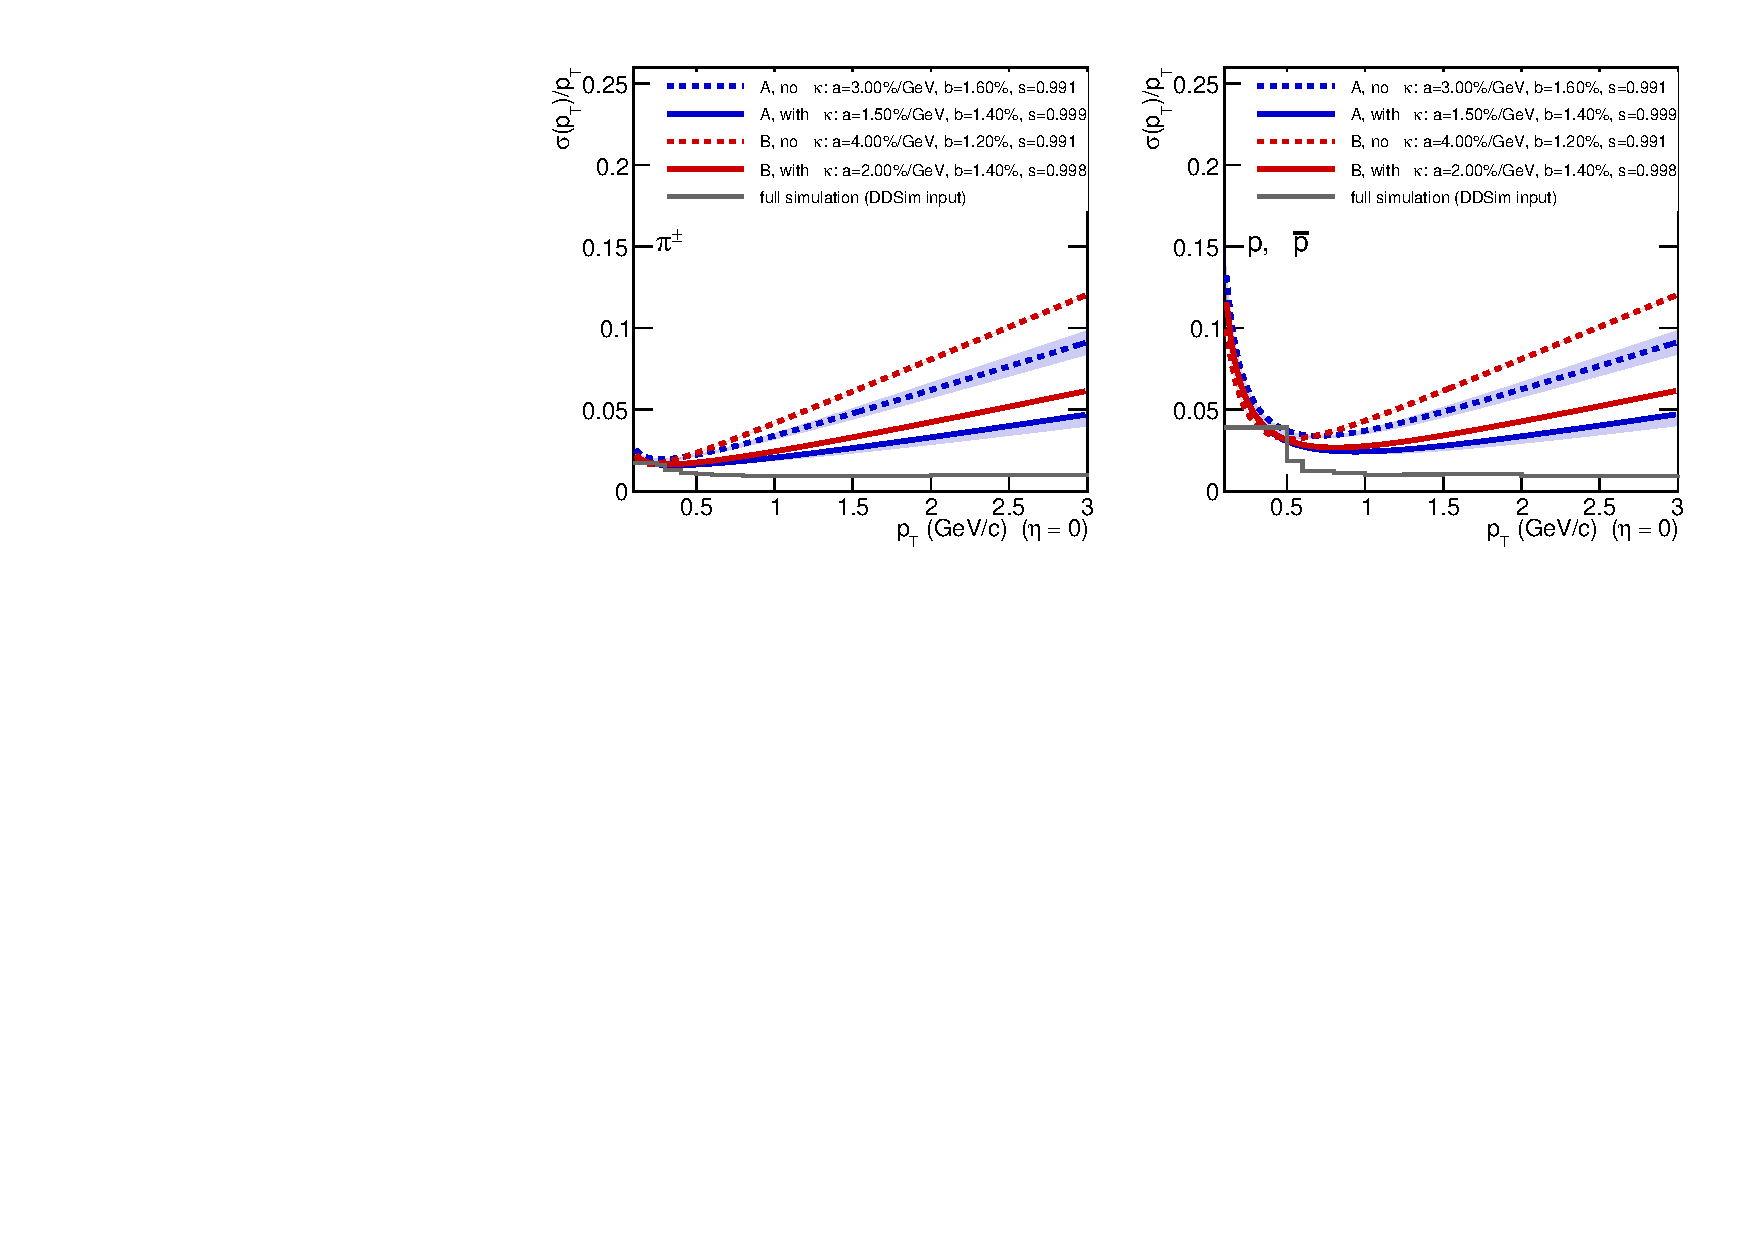
\includegraphics[width=\textwidth]{fig_res}
\caption{Fitted $\sigma(\pt)/\pt$ at $\eta=0$ (Eq.~\ref{eq:model}) for pions (left) and protons (right): period A (blue) and B
(red), without (dashed) and with (solid) $\kappa$; lines at the \Ks{} best point (Table~\ref{tab:summary}), bands = envelope of the $(a,b)$ grid nodes with
\Ks{} $\Delta\chi^2<2.3$ (profiled over $s$; \ResBandNote). Grey: full-simulation
response of the DDSim input. Script \fpath{scripts/plot_res.C}.}
\label{fig:res}
\end{figure}

For pions at 1, 2, 3\gevc: period A \PerARawResPiOne, \PerARawResPiTwo, \PerARawResPiThree\% without and \PerAKapResPiOne,
\PerAKapResPiTwo, \PerAKapResPiThree\% with $\kappa$; period B \PerBRawResPiOne, \PerBRawResPiTwo, \PerBRawResPiThree\% and
\PerBKapResPiOne, \PerBKapResPiTwo, \PerBKapResPiThree\%. Above $\approx1.5$\gevc{} the curves are constrained mainly by the two
highest \Ks{} bins (Table~\ref{tab:entries}).

\begin{figure}[H]
\centering
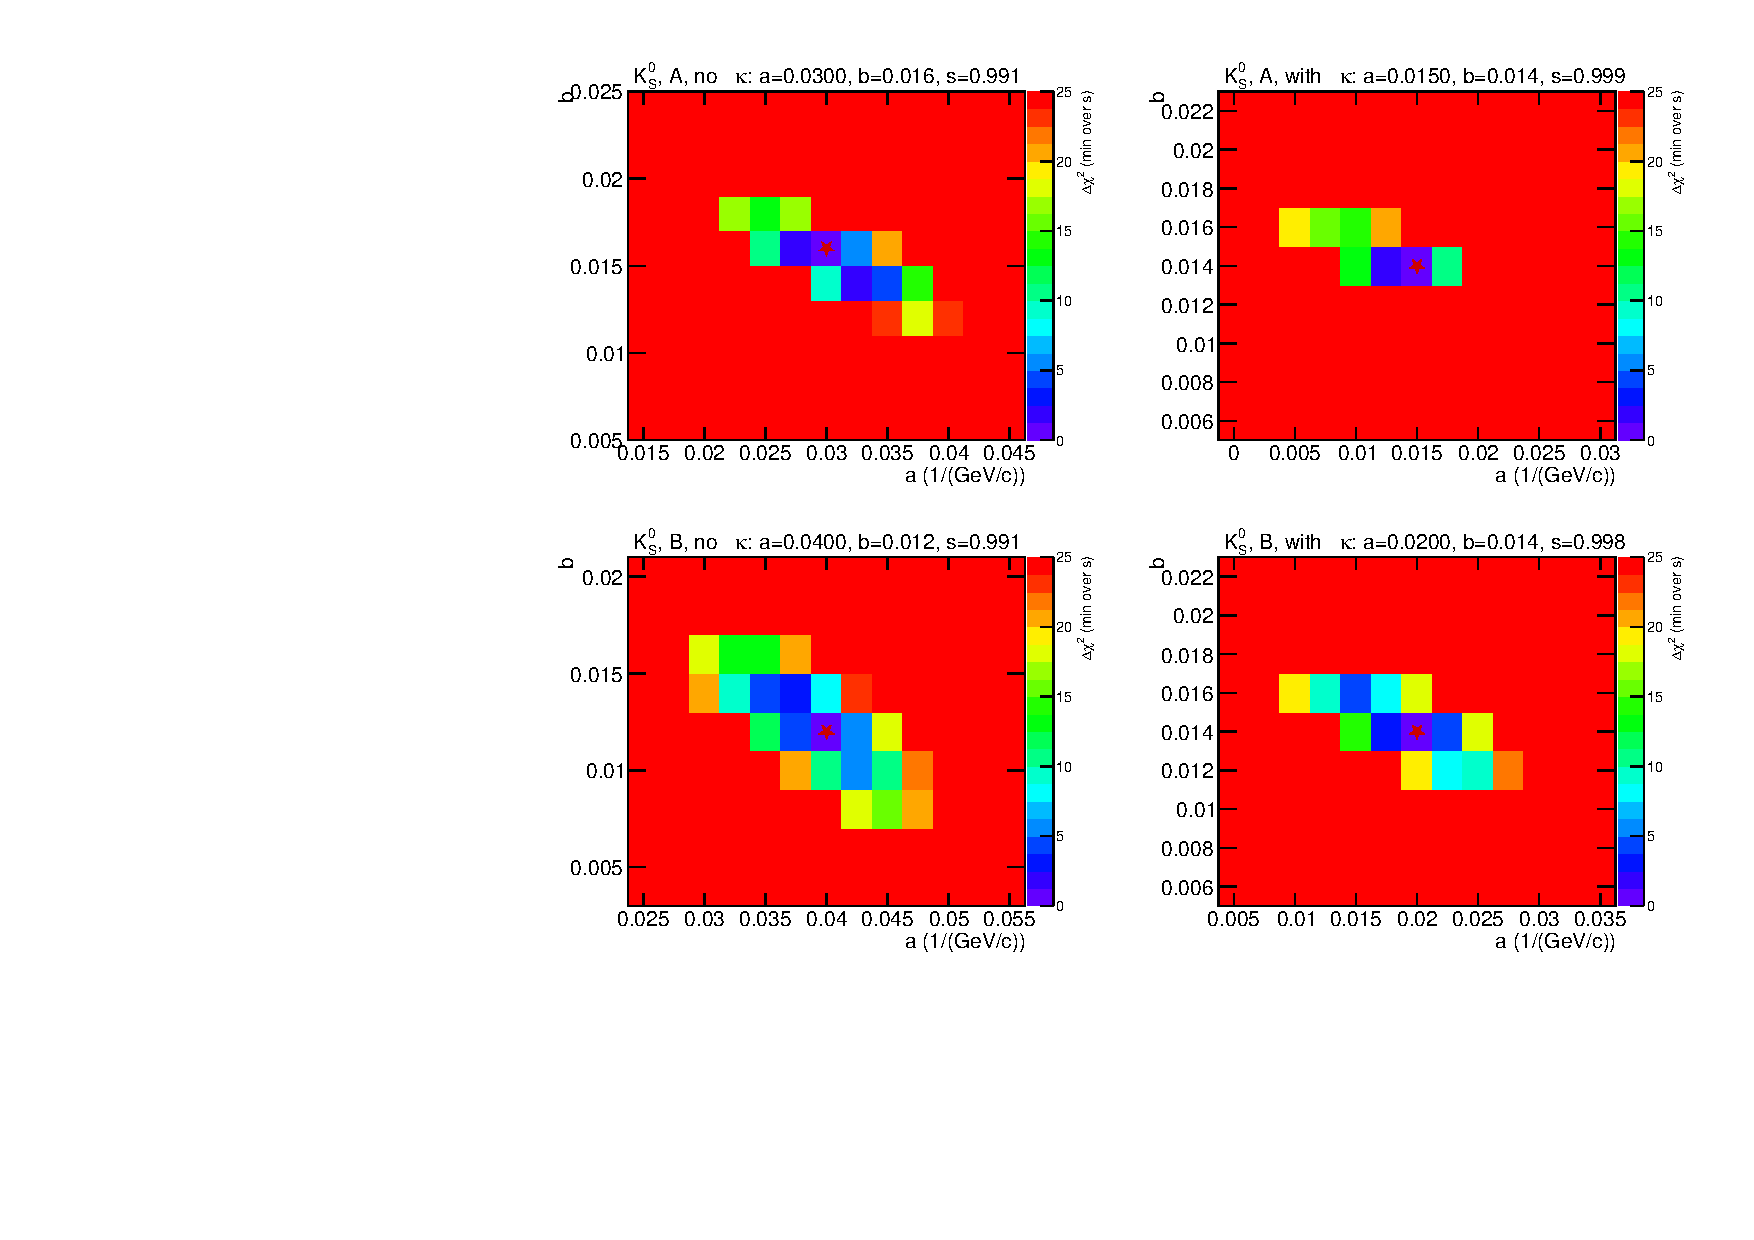
\includegraphics[width=0.92\textwidth]{fig_chi2}
\caption{$\Delta\chi^2$ of the \Ks{} fit in the $(a,b)$ plane, minimised over $s$, on the grid nodes (cells; colour scale
capped at 25): period A (top) and B (bottom), without (left) and with (right) $\kappa$. Red star: best node. The $\Delta\chi^2<2.3$ region is only a few nodes wide, so the
grid step (0.0025 in $a$, 0.002 in $b$) limits the resolution of the intervals. Each panel shows $\pm0.016$~(GeV/$c$)$^{-1}$ in $a$ and $\pm0.009$ in $b$ around its best node.}
\label{fig:chi2}
\end{figure}

\subsection{Invariant-mass distributions before and after the correction}
\label{sec:massdist}

Figure~\ref{fig:massdist} compares the \pt-integrated mass distributions of the same QA-selected candidates, recomputed from the
daughter momenta without $\kappa$ (blue) and with $\kappa$ (red); the KFParticle mass is shown for reference (grey). Only the
daughter \pt{} changes; $\eta$, $\varphi$ and the selection are the same. Figures~\ref{fig:massdistKsA}--\ref{fig:massdistLaB}
show the same per V0-\pt{} bin of the momentum fit (the V0 \pt{} is that of each version, so a candidate can change bin).

\begin{itemize}
\item \Ks: with $\kappa$ the peak moves up towards the PDG mass and becomes narrower and higher in both periods (Gaussian fit,
  Table~\ref{tab:peaksks}: mean \PerARawKsGM{} $\to$ \PerAKapKsGM, $\sigma$ \PerARawKsGS{} $\to$ \PerAKapKsGS\mevcc{} in A;
  \PerBRawKsGM{} $\to$ \PerBKapKsGM, \PerBRawKsGS{} $\to$ \PerBKapKsGS\mevcc{} in B). The change is largest above
  1.2\gevc, where the uncorrected peak is broad and the corrected one narrow.
\item \La: mean \PerARawLaGM{} $\to$ \PerAKapLaGM, $\sigma$ \PerARawLaGS{} $\to$ \PerAKapLaGS\mevcc{} (A) and
  \PerBRawLaGM{} $\to$ \PerBKapLaGM, \PerBRawLaGS{} $\to$ \PerBKapLaGS\mevcc{} (B), PDG \PdgLa\mevcc. The narrowing is smaller in
  absolute terms than for \Ks, as expected from the small \La{} decay momentum (the mass is less sensitive to the daughter momenta).
\item The background is the same in both recomputed versions. The number of entries in the plotted mass range differs by less than 1\%
  between them (\Ks{} A \PerAKsMdRaw{} vs \PerAKsMdKap, B \PerBKsMdRaw{} vs \PerBKsMdKap), as expected since the correction
  only moves masses by a few \mevcc.
\item The KFParticle mass has more combinatorial background in the same mass window (the recomputed spectra contain
  \PerAKsMdRatio{} (A) and \PerBKsMdRatio{} (B) of the KFP \Ks{} entries, \PerALaMdRatio{} and \PerBLaMdRatio{} for \La{}),
  although the candidates are the same. The cause is not investigated (open issue~3).
\end{itemize}

\begin{figure}[H]
\centering
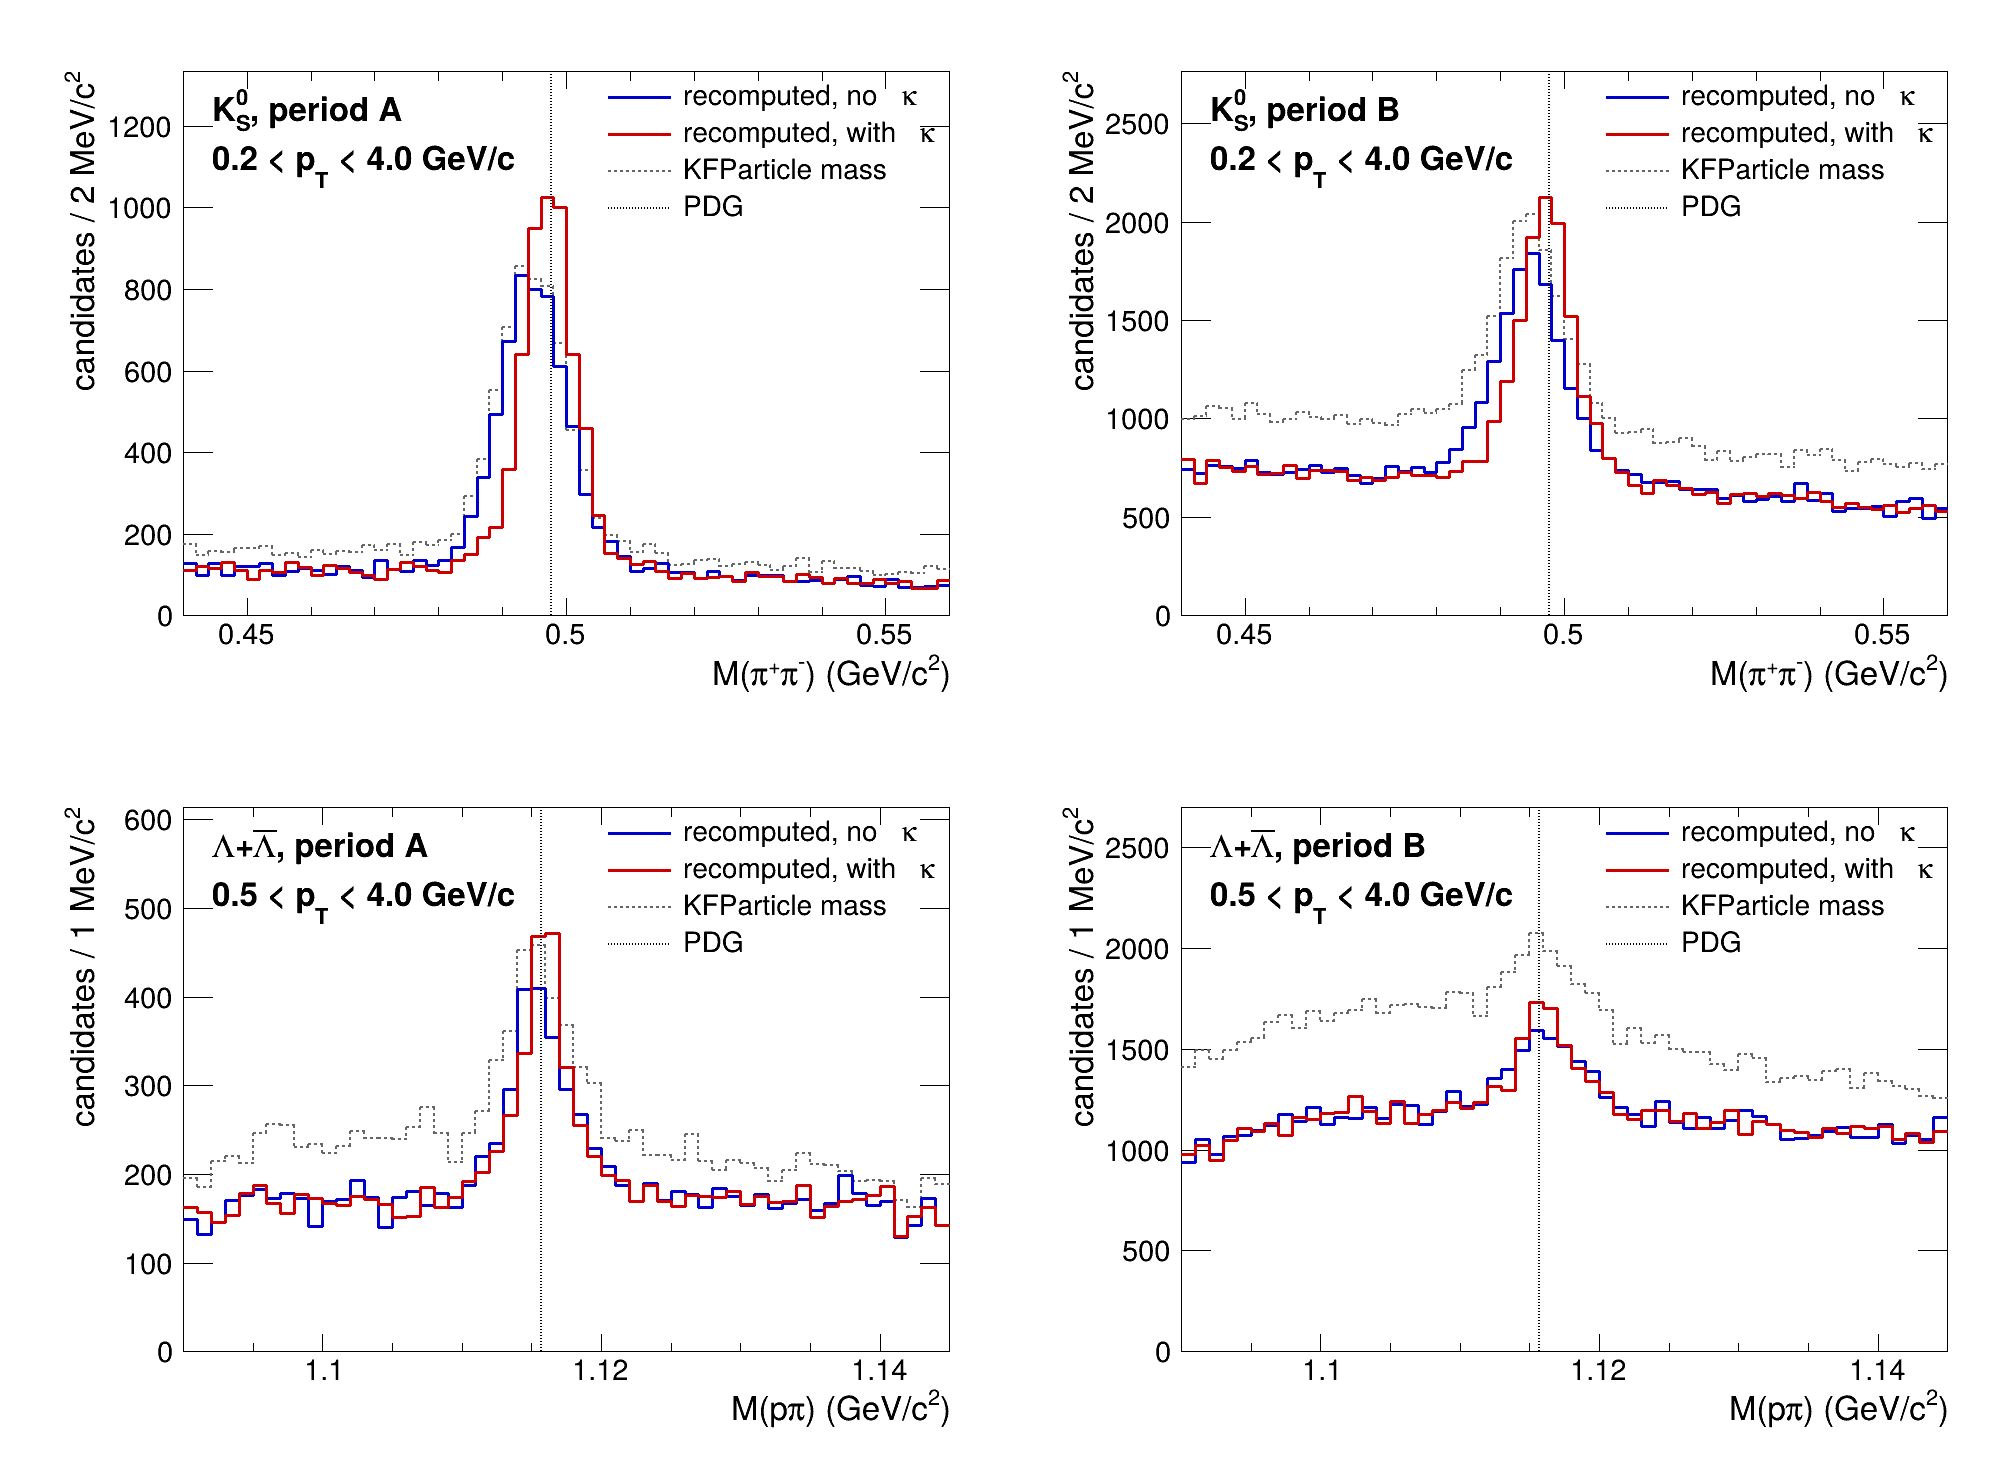
\includegraphics[width=\textwidth]{fig_massdist_int}
\caption{Invariant-mass distributions, \pt-integrated (\Ks{} $0.2<\pt<4.0$, \La+$\bar\Lambda$ $0.5<\pt<4.0$\gevc), period A
(left) and B (right): recomputed without $\kappa$ (blue), with $\kappa$ (red), KFParticle mass (grey dashed); dotted line: PDG
mass. Same QA-selected candidates in all curves. Script \fpath{scripts/massdist.C}.}
\label{fig:massdist}
\end{figure}

\begin{figure}[H]
\centering
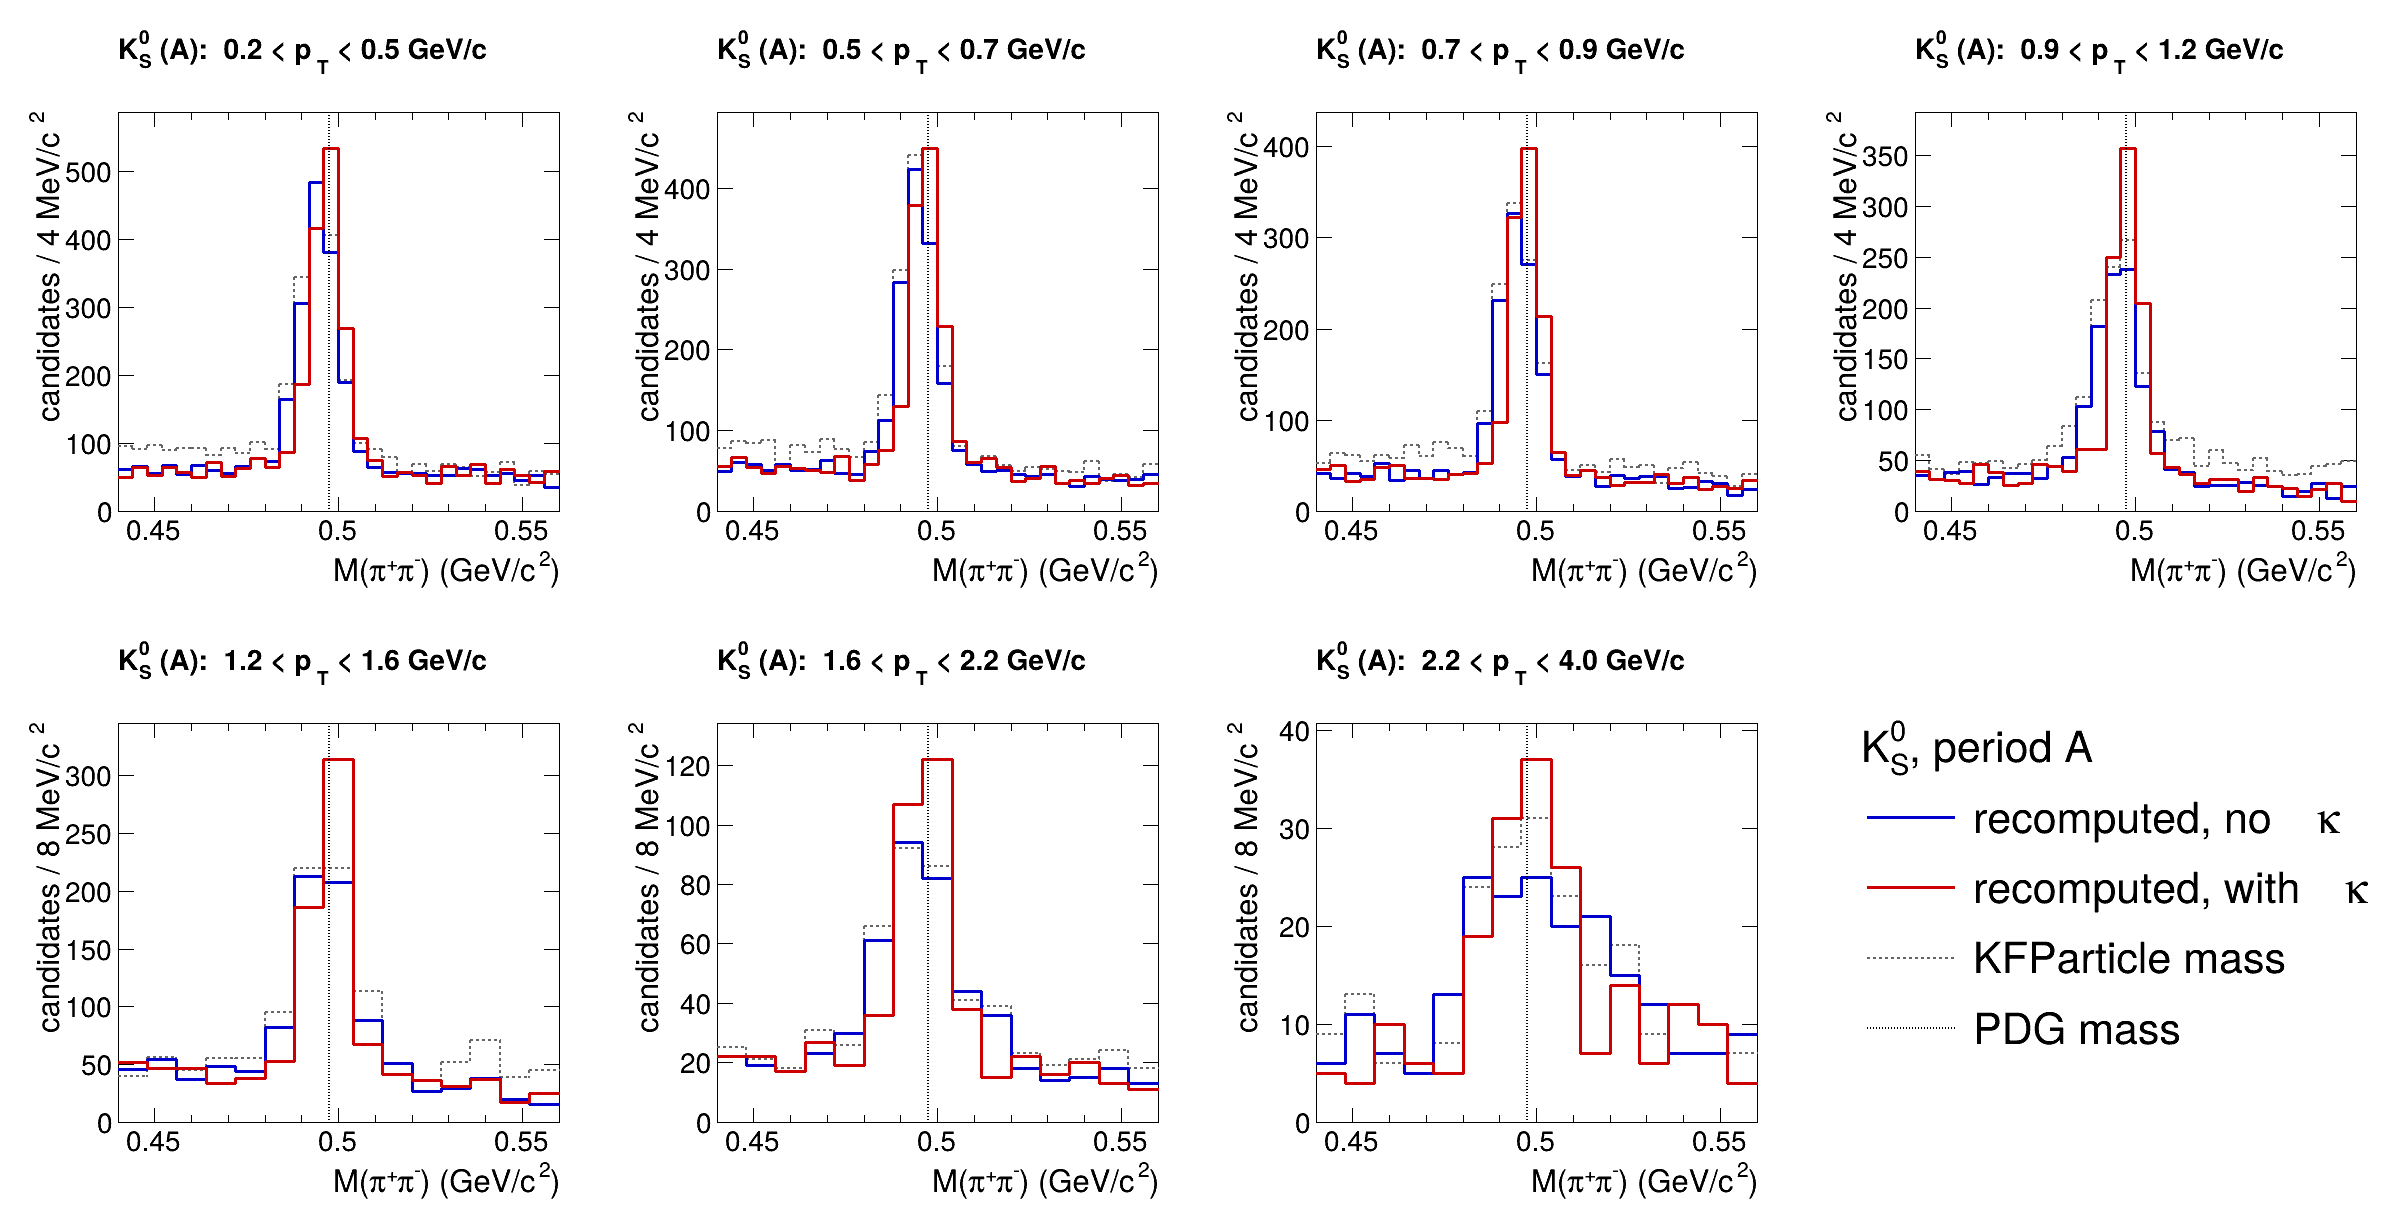
\includegraphics[width=\textwidth]{fig_massdist_Ks_A}
\caption{\Ks{} mass per V0-\pt{} bin, period A, without (blue) and with (red) $\kappa$, KFParticle mass (grey dashed). Bin width
2, 4 or 8\mevcc{} depending on the statistics of the panel (axis title).}
\label{fig:massdistKsA}
\end{figure}

\begin{figure}[H]
\centering
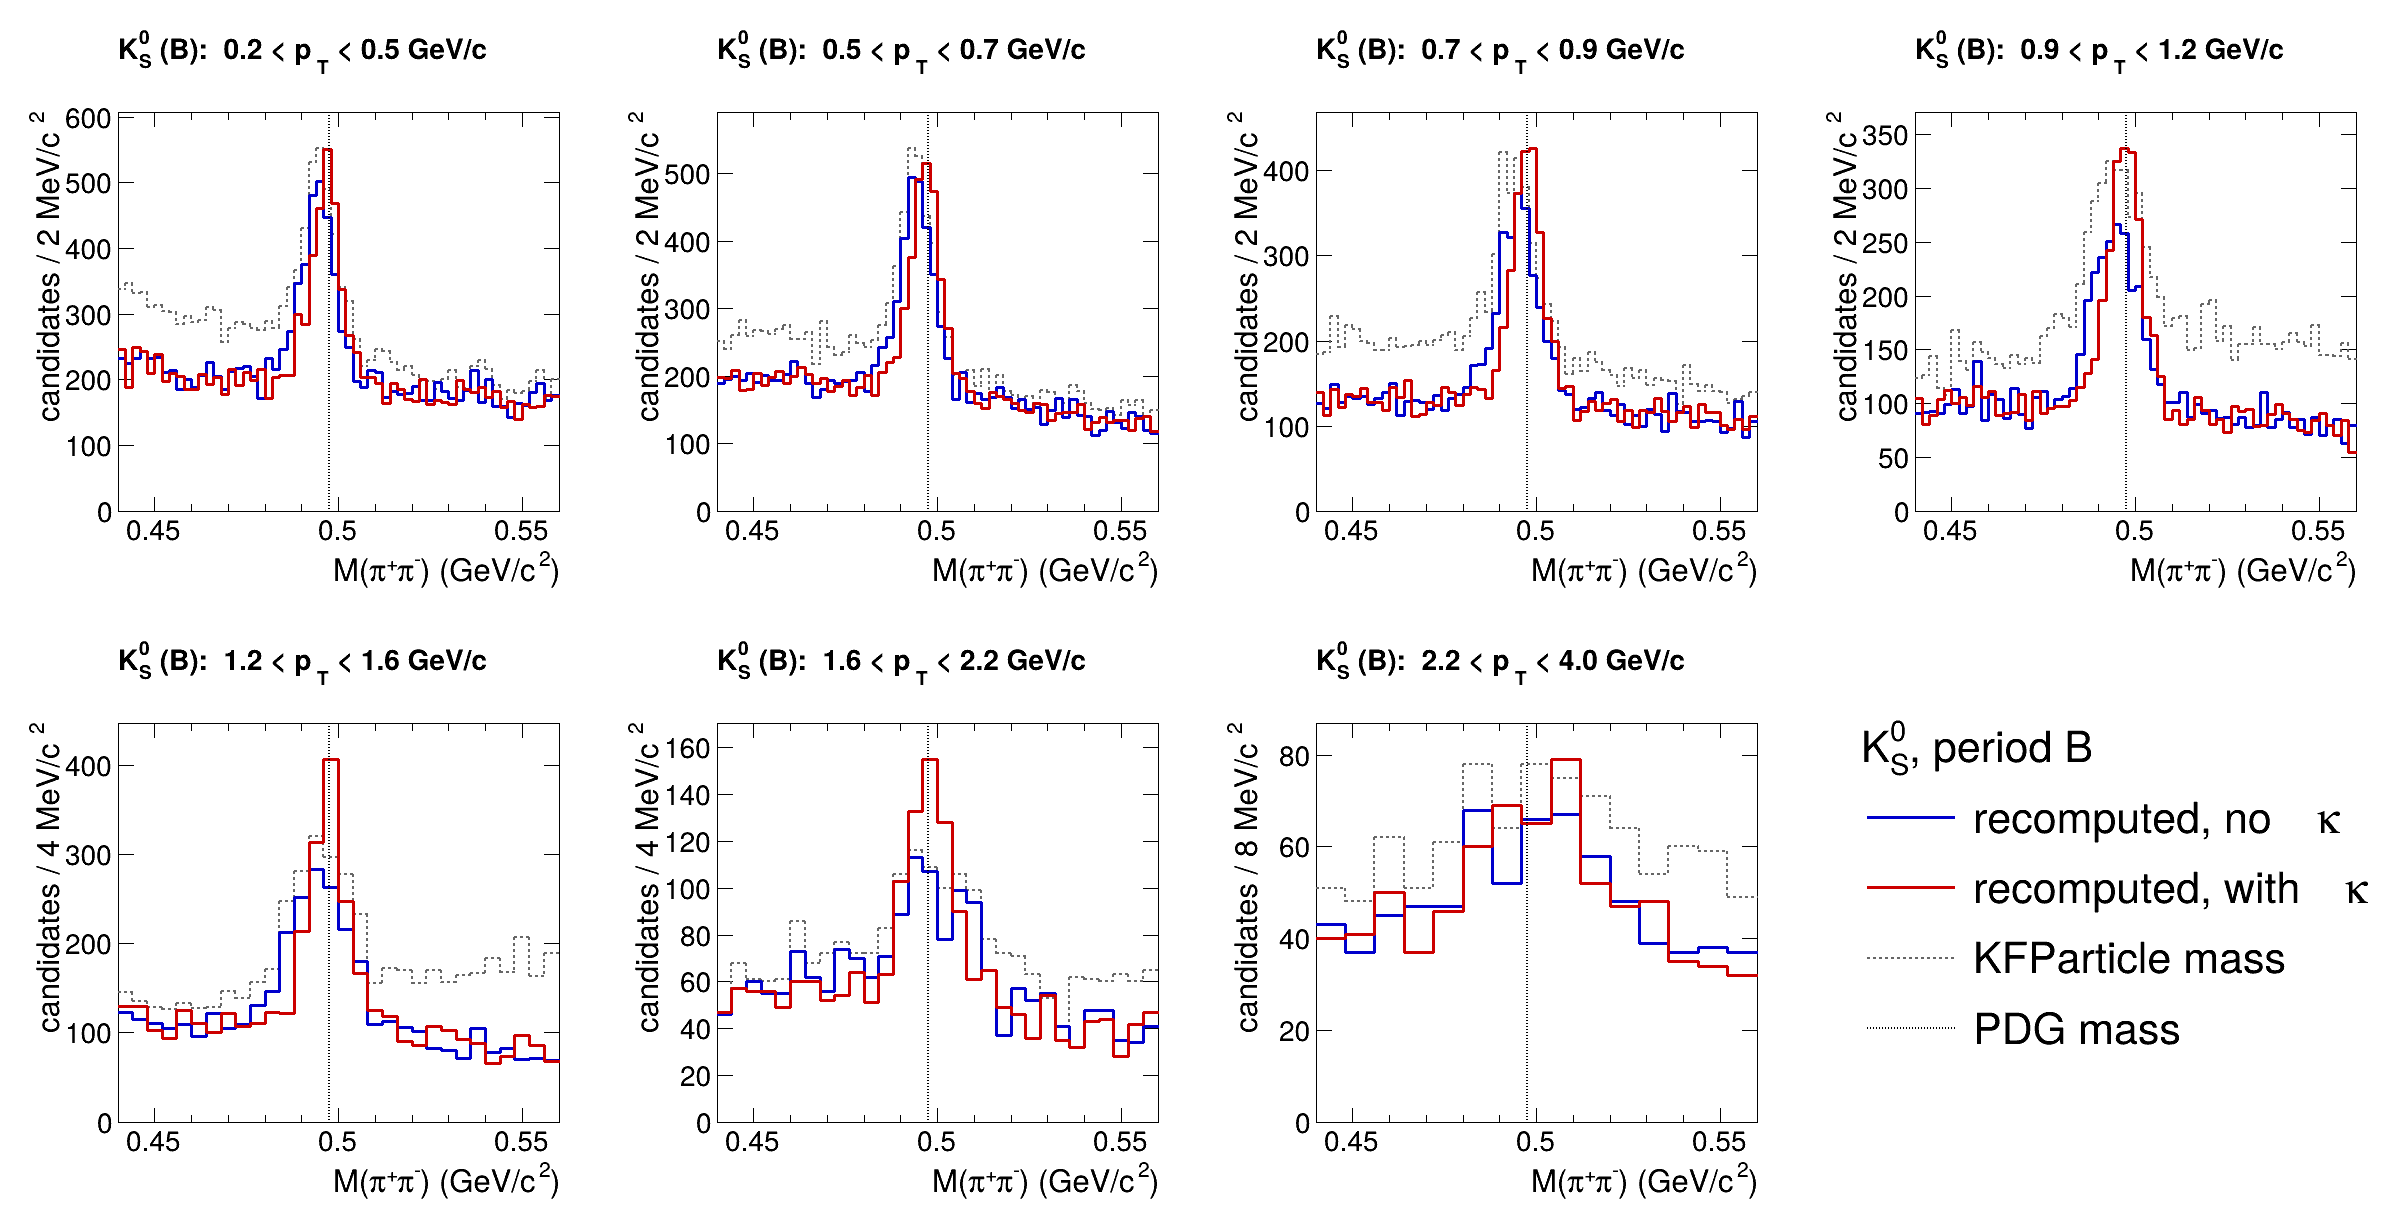
\includegraphics[width=\textwidth]{fig_massdist_Ks_B}
\caption{As Fig.~\ref{fig:massdistKsA}, period B.}
\label{fig:massdistKsB}
\end{figure}

\begin{figure}[H]
\centering
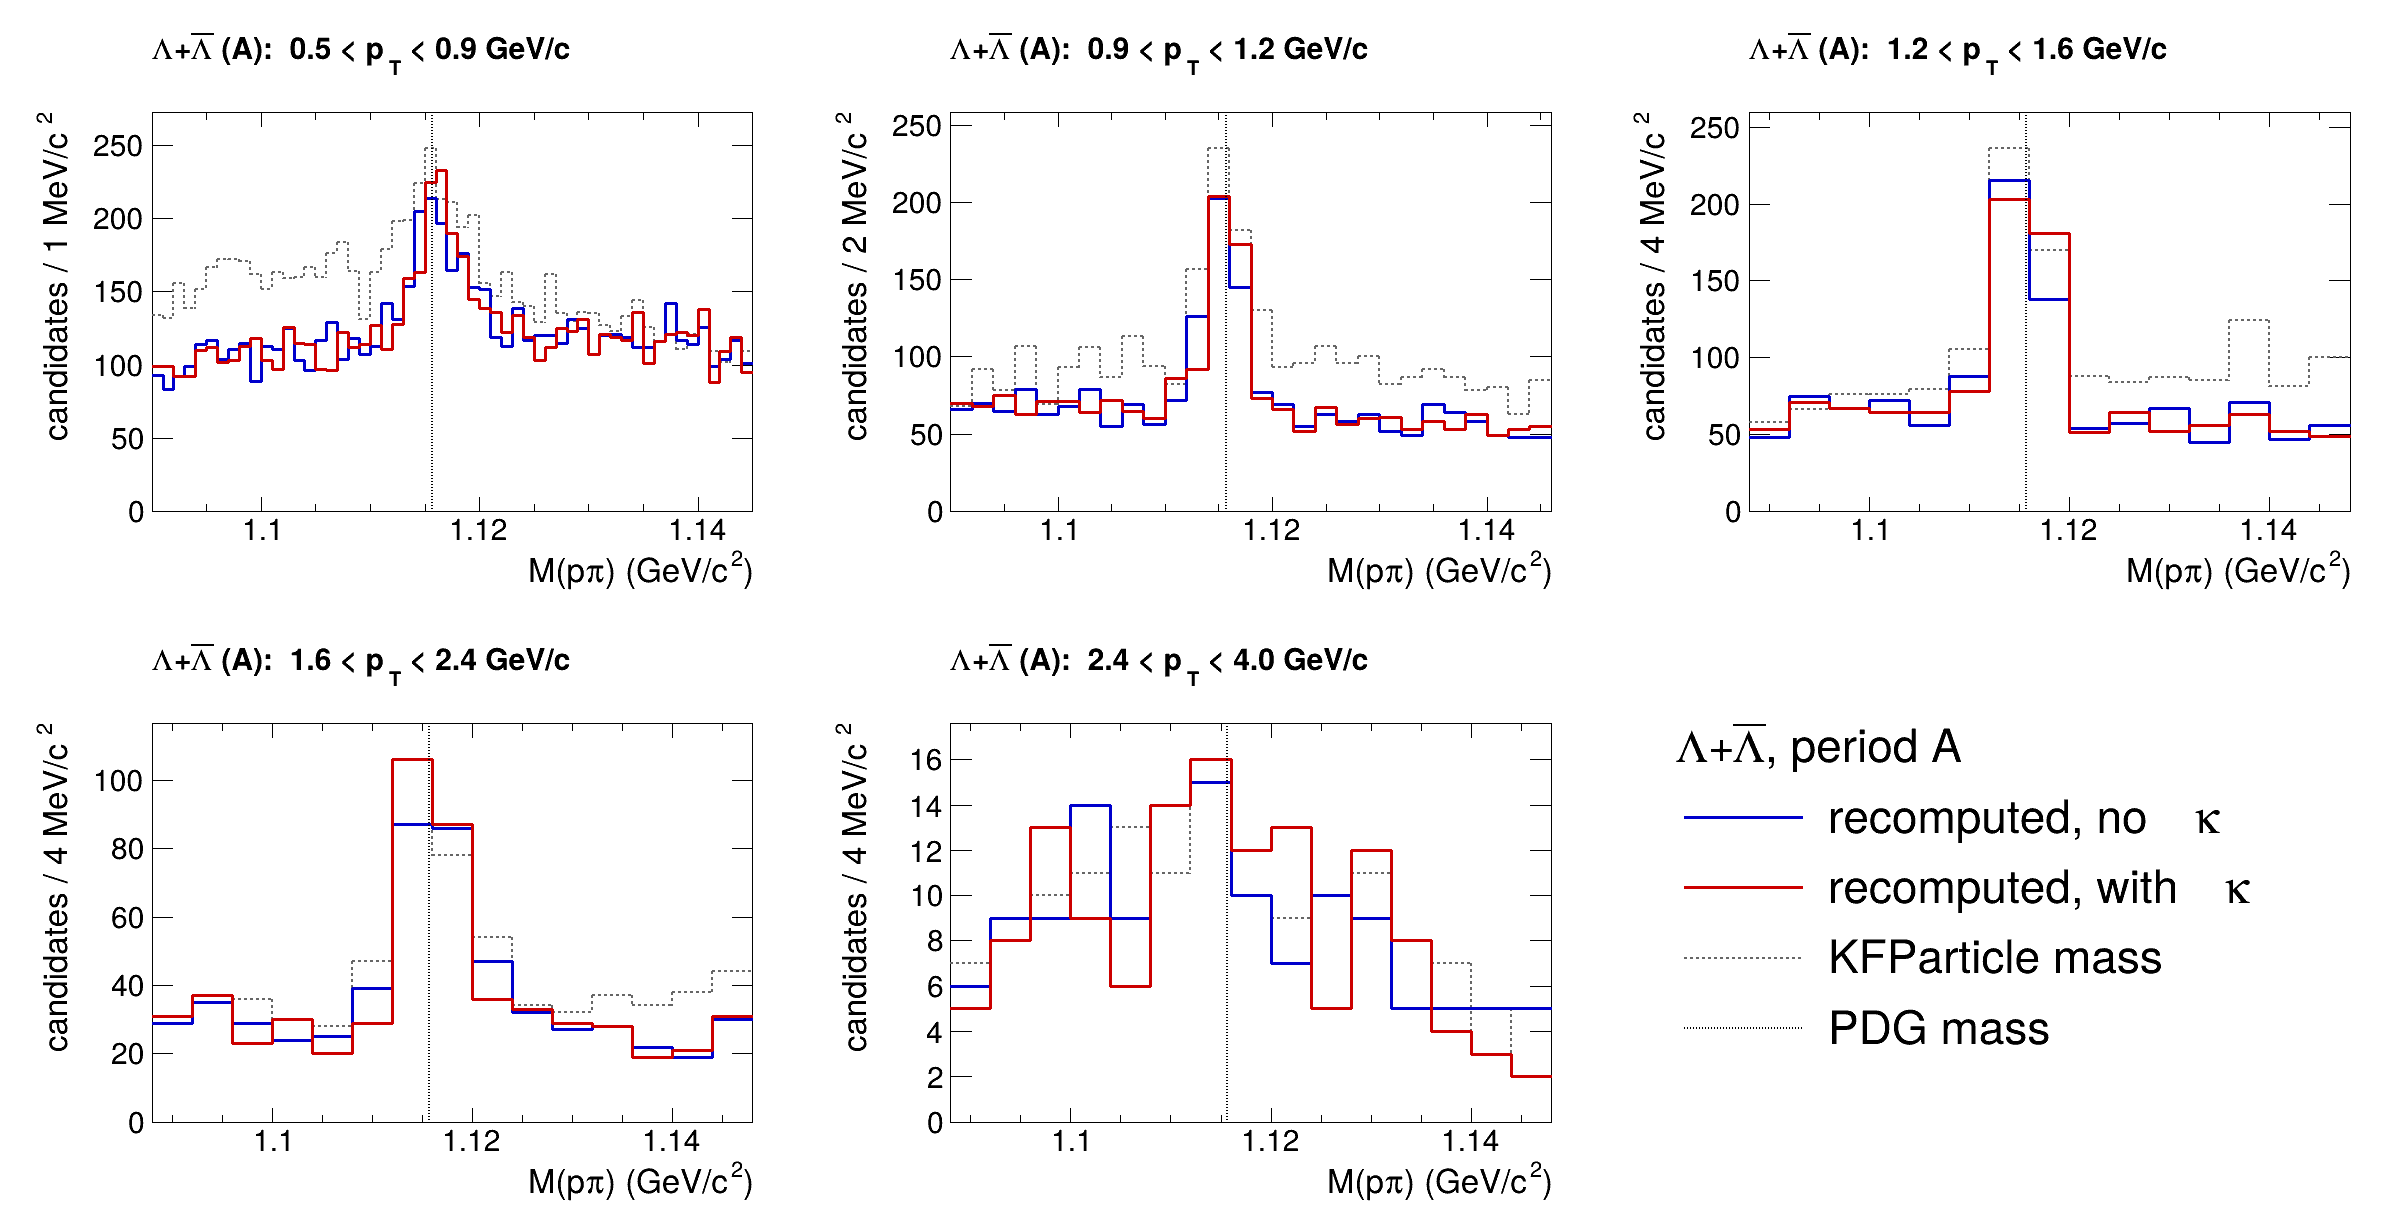
\includegraphics[width=\textwidth]{fig_massdist_La_A}
\caption{\La+$\bar\Lambda$ mass per V0-\pt{} bin, period A, without (blue) and with (red) $\kappa$, KFParticle mass (grey dashed).
Bin width 1, 2 or 4\mevcc{} depending on the statistics of the panel.}
\label{fig:massdistLaA}
\end{figure}

\begin{figure}[H]
\centering
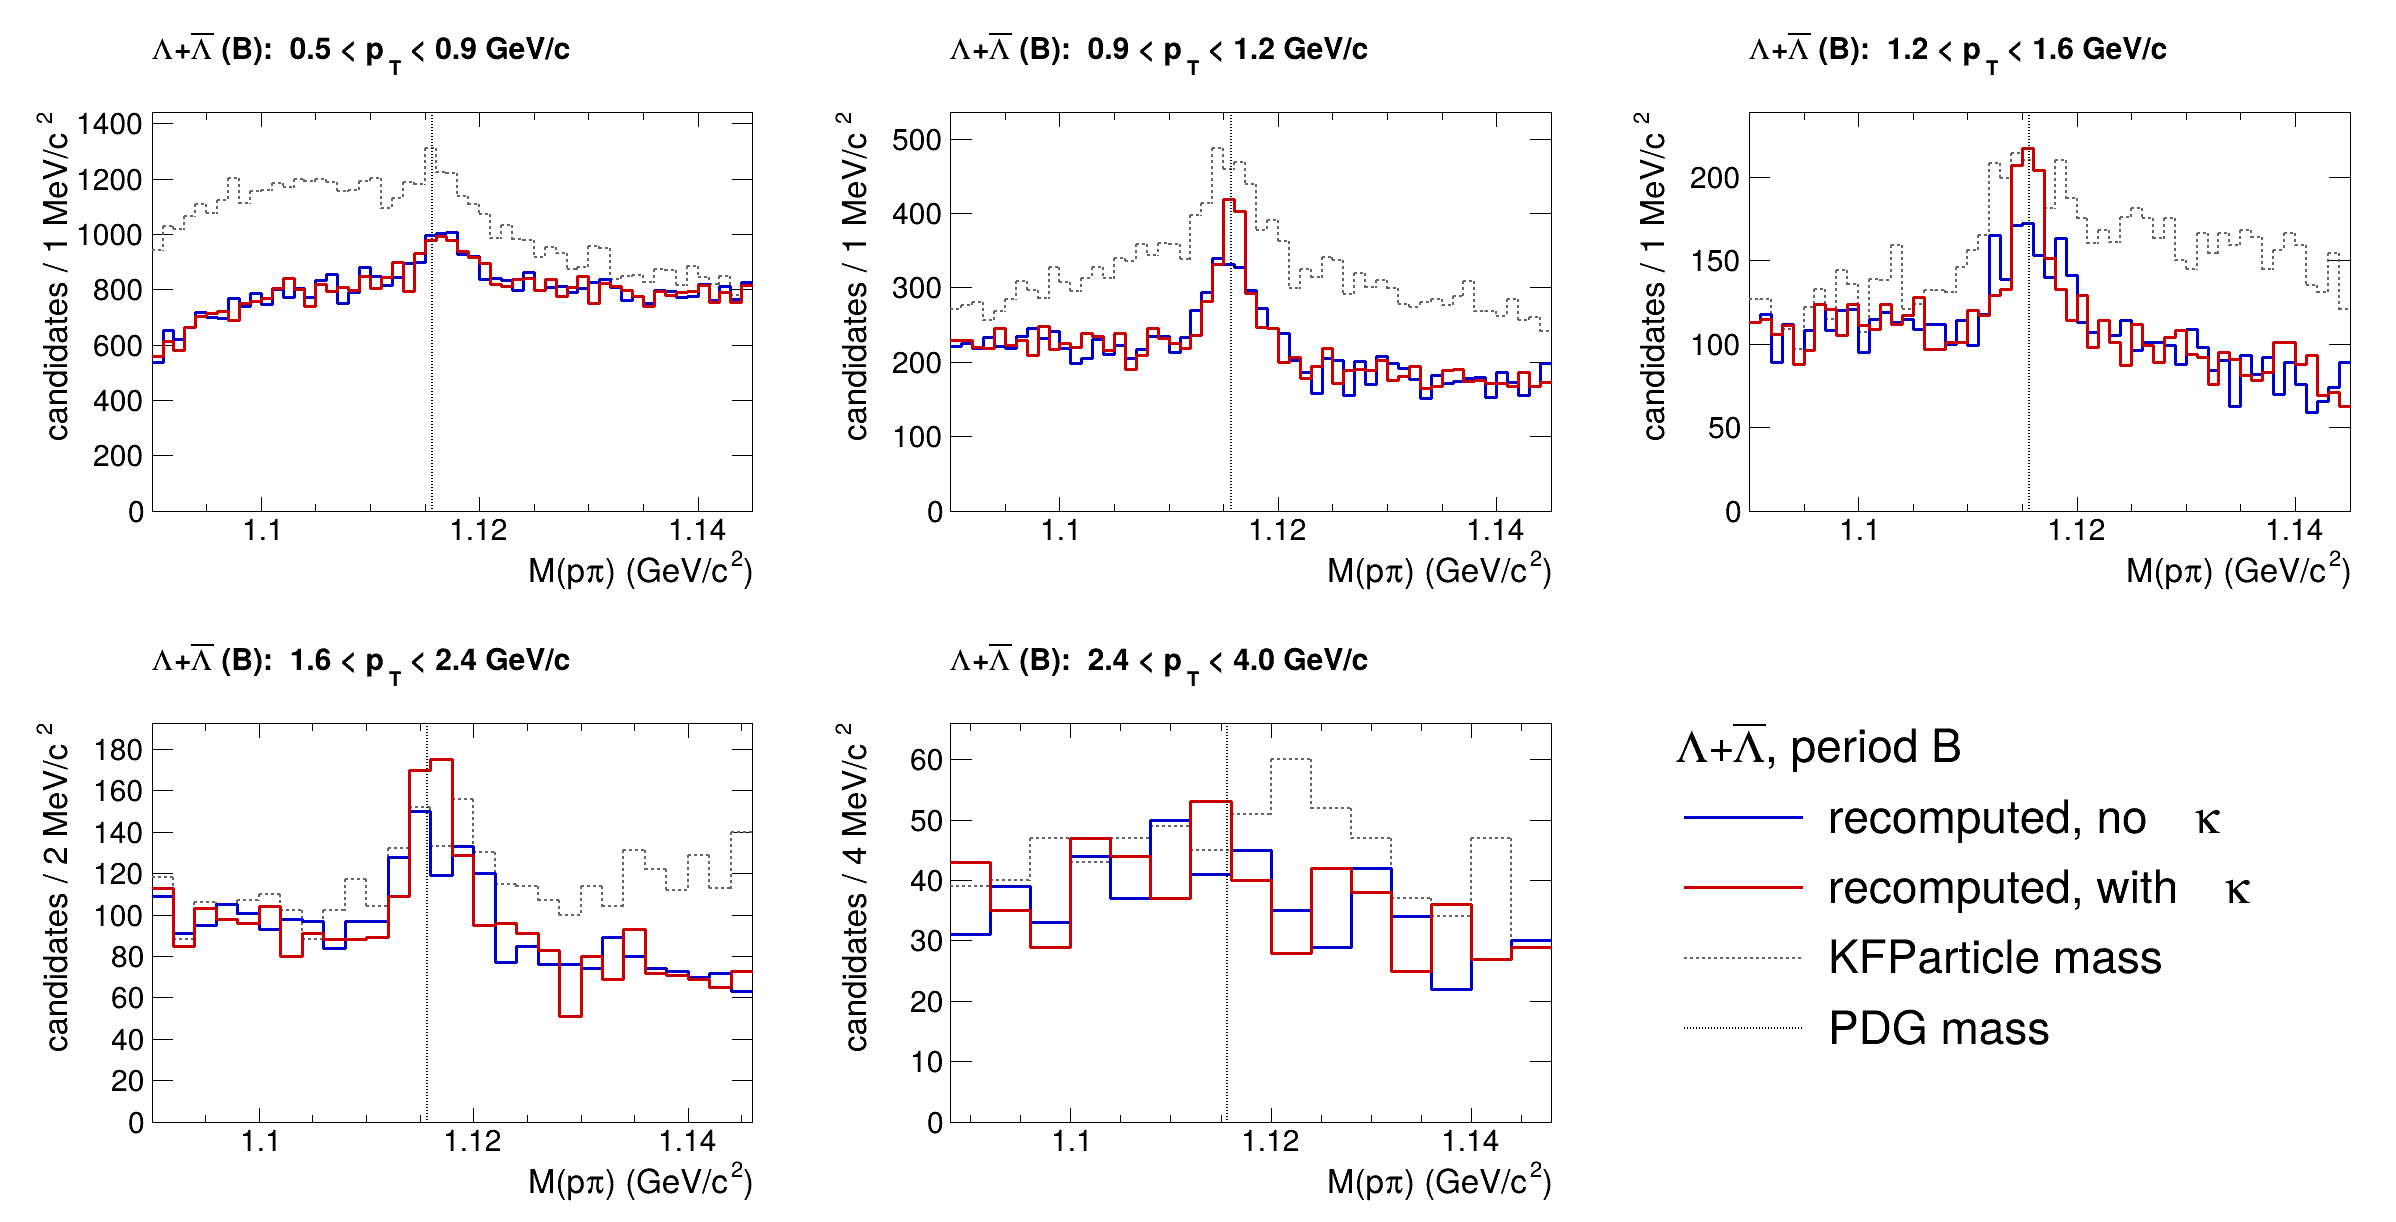
\includegraphics[width=\textwidth]{fig_massdist_La_B}
\caption{As Fig.~\ref{fig:massdistLaA}, period B.}
\label{fig:massdistLaB}
\end{figure}

\subsection{Mass peaks}

\begin{figure}[H]
\centering
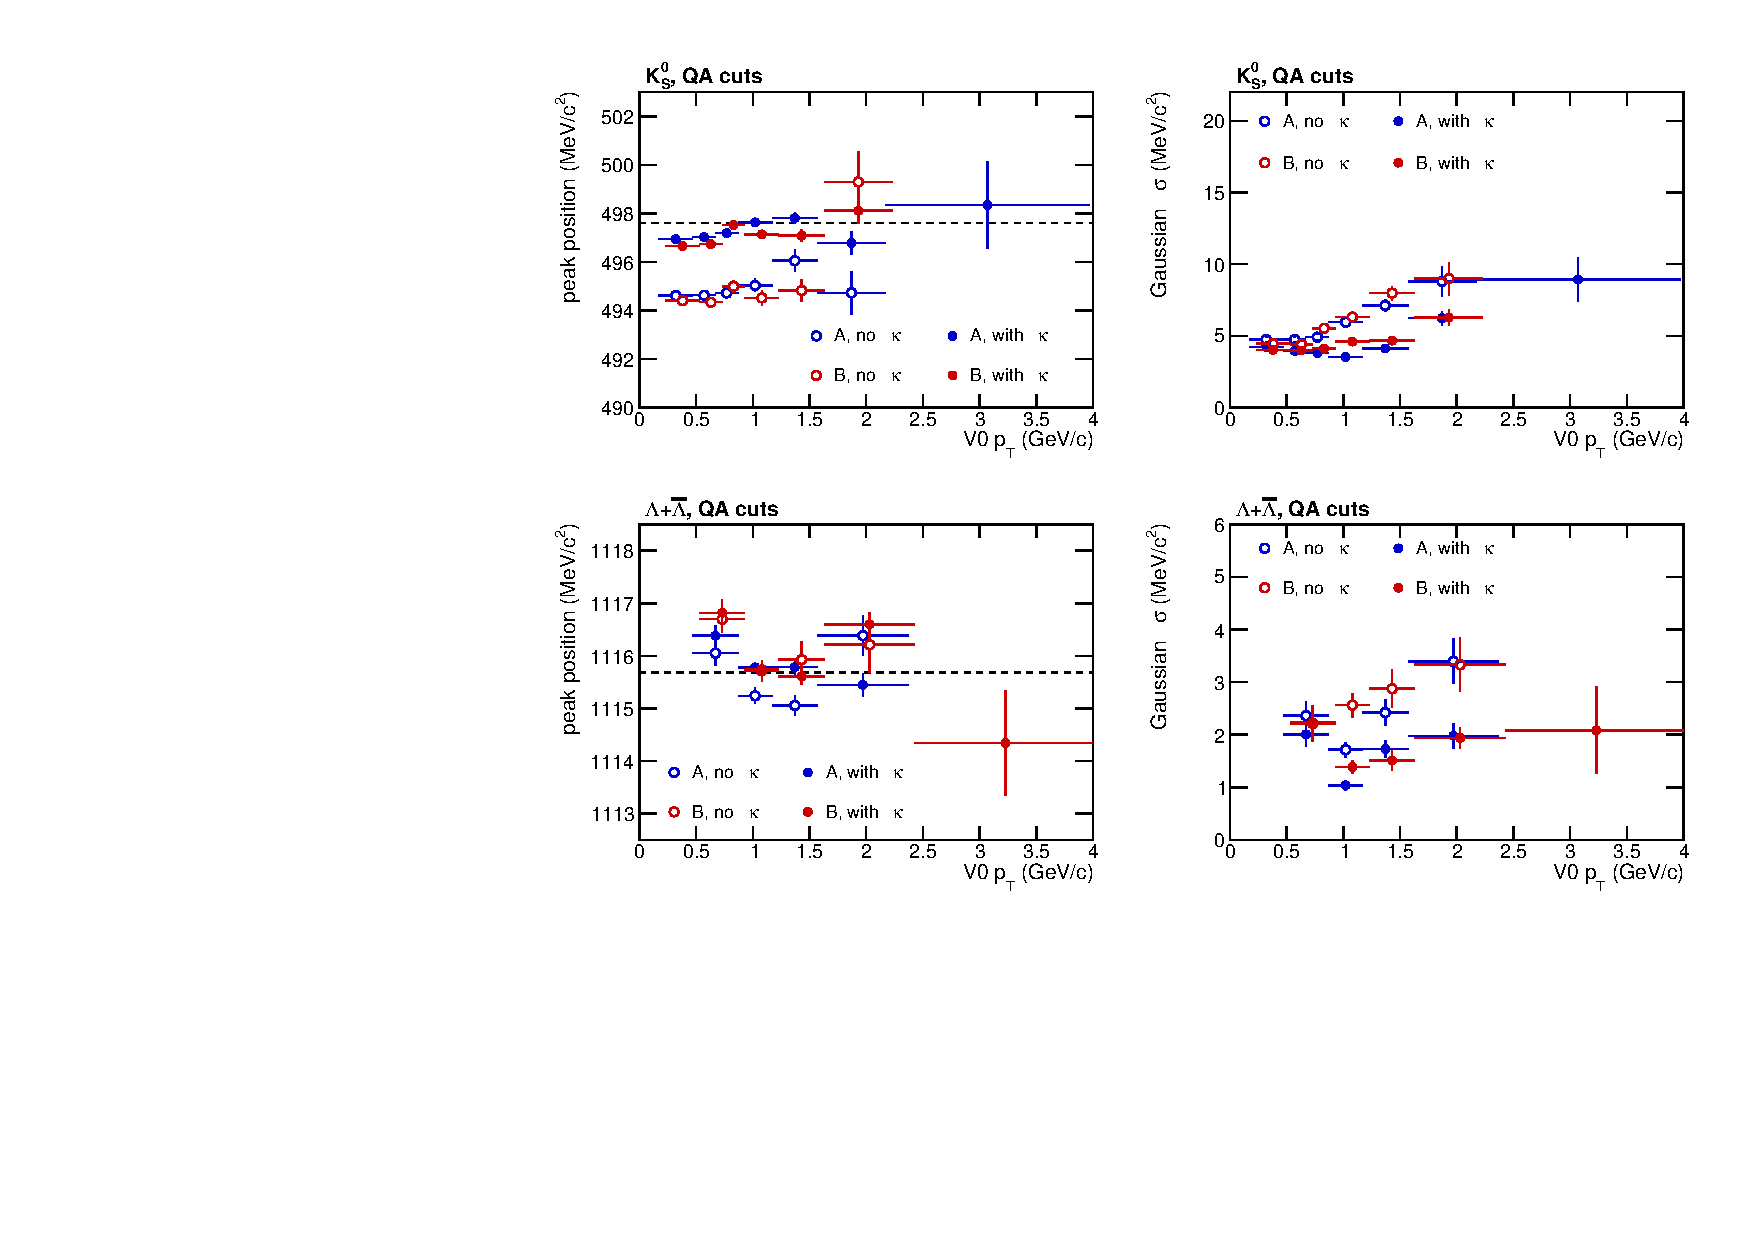
\includegraphics[width=\textwidth]{fig_peaks}
\caption{Gaussian peak position (left) and width (right) per V0-\pt{} bin for \Ks{} (top; Gaussian + linear, 0.46--0.54~GeV/$c^2$)
and \La+$\bar\Lambda$ (bottom; Gaussian + quadratic, 1.103--1.130~GeV/$c^2$): period A (blue) and B (red), without (open) and
with (full) $\kappa$; points of the two periods are offset by $\pm0.03$\gevc{} for visibility. Dashed: PDG mass. Unconstrained fits
(mean error $>2$\mevcc{} or width error $>60\%$) are not drawn. Display only; the calibration uses the template fit.
Script \fpath{scripts/peaks.C}.}
\label{fig:peaks}
\end{figure}

\begin{table}[H]
\centering\footnotesize
\caption{\Ks{} Gaussian peak position $M$ and width $\sigma$ (MeV/$c^2$) per V0-\pt{} bin (GeV/$c$), fits of
Fig.~\ref{fig:peaks}; ``--'' unconstrained. PDG \PdgKs\mevcc.}
\label{tab:peaksks}
\setlength{\tabcolsep}{2.4pt}
\begin{tabular}{lcccccccc}
\toprule
 & \multicolumn{4}{c}{period A} & \multicolumn{4}{c}{period B} \\
\pt & $M$, no $\kappa$ & $\sigma$, no $\kappa$ & $M$, $\kappa$ & $\sigma$, $\kappa$ & $M$, no $\kappa$ & $\sigma$, no $\kappa$ & $M$, $\kappa$ & $\sigma$, $\kappa$ \\
\midrule
% generated by scripts/make_numbers.py
0.2--0.5 & 494.61$\pm$0.17 & 4.74$\pm$0.16 & 496.94$\pm$0.15 & 4.23$\pm$0.15 & 494.41$\pm$0.20 & 4.46$\pm$0.22 & 496.65$\pm$0.18 & 4.02$\pm$0.20 \\
0.5--0.7 & 494.63$\pm$0.18 & 4.75$\pm$0.17 & 497.02$\pm$0.15 & 3.96$\pm$0.15 & 494.34$\pm$0.19 & 4.42$\pm$0.20 & 496.73$\pm$0.16 & 3.98$\pm$0.17 \\
0.7--0.9 & 494.72$\pm$0.20 & 4.91$\pm$0.18 & 497.19$\pm$0.15 & 3.80$\pm$0.13 & 494.99$\pm$0.24 & 5.53$\pm$0.27 & 497.53$\pm$0.17 & 4.11$\pm$0.17 \\
0.9--1.2 & 495.03$\pm$0.27 & 5.95$\pm$0.27 & 497.64$\pm$0.15 & 3.53$\pm$0.14 & 494.52$\pm$0.30 & 6.32$\pm$0.30 & 497.14$\pm$0.19 & 4.60$\pm$0.19 \\
1.2--1.6 & 496.05$\pm$0.45 & 7.12$\pm$0.39 & 497.81$\pm$0.23 & 4.12$\pm$0.23 & 494.82$\pm$0.46 & 7.99$\pm$0.49 & 497.09$\pm$0.25 & 4.67$\pm$0.28 \\
1.6--2.2 & 494.73$\pm$0.89 & 8.79$\pm$1.03 & 496.79$\pm$0.48 & 6.24$\pm$0.48 & 499.30$\pm$1.25 & 9.00$\pm$1.15 & 498.11$\pm$0.51 & 6.27$\pm$0.56 \\
2.2--4.0 & -- & -- & 498.34$\pm$1.78 & 8.92$\pm$1.55 & -- & -- & -- & -- \\
0.2--4.0 (all) & 494.78$\pm$0.10 & 5.30$\pm$0.10 & 497.21$\pm$0.07 & 4.03$\pm$0.07 & 494.57$\pm$0.11 & 5.43$\pm$0.13 & 497.04$\pm$0.08 & 4.33$\pm$0.09 \\

\bottomrule
\end{tabular}
\end{table}

\begin{table}[H]
\centering\footnotesize
\caption{As Table~\ref{tab:peaksks} for \La+$\bar\Lambda$. PDG \PdgLa\mevcc.}
\label{tab:peaksla}
\setlength{\tabcolsep}{2.4pt}
\begin{tabular}{lcccccccc}
\toprule
 & \multicolumn{4}{c}{period A} & \multicolumn{4}{c}{period B} \\
\pt & $M$, no $\kappa$ & $\sigma$, no $\kappa$ & $M$, $\kappa$ & $\sigma$, $\kappa$ & $M$, no $\kappa$ & $\sigma$, no $\kappa$ & $M$, $\kappa$ & $\sigma$, $\kappa$ \\
\midrule
% generated by scripts/make_numbers.py
0.5--0.9 & 1116.05$\pm$0.24 & 2.36$\pm$0.28 & 1116.38$\pm$0.19 & 2.01$\pm$0.24 & 1116.70$\pm$0.26 & 2.21$\pm$0.35 & 1116.82$\pm$0.25 & 2.24$\pm$0.32 \\
0.9--1.2 & 1115.24$\pm$0.15 & 1.72$\pm$0.14 & 1115.78$\pm$0.10 & 1.04$\pm$0.09 & 1115.72$\pm$0.20 & 2.56$\pm$0.23 & 1115.75$\pm$0.10 & 1.39$\pm$0.13 \\
1.2--1.6 & 1115.06$\pm$0.20 & 2.42$\pm$0.24 & 1115.79$\pm$0.14 & 1.73$\pm$0.17 & 1115.93$\pm$0.35 & 2.88$\pm$0.36 & 1115.61$\pm$0.15 & 1.51$\pm$0.18 \\
1.6--2.4 & 1116.39$\pm$0.38 & 3.40$\pm$0.43 & 1115.45$\pm$0.22 & 1.98$\pm$0.24 & 1116.21$\pm$0.52 & 3.33$\pm$0.51 & 1116.60$\pm$0.22 & 1.94$\pm$0.19 \\
2.4--4.0 & -- & -- & -- & -- & -- & -- & 1114.34$\pm$1.00 & 2.08$\pm$0.83 \\
0.5--4.0 (all) & 1115.55$\pm$0.12 & 2.16$\pm$0.14 & 1115.92$\pm$0.08 & 1.63$\pm$0.11 & 1116.24$\pm$0.16 & 2.69$\pm$0.19 & 1116.11$\pm$0.10 & 1.88$\pm$0.13 \\

\bottomrule
\end{tabular}
\end{table}

\subsection{Template fits per V0-\pt{} bin}

Figures~\ref{fig:massksA}--\ref{fig:masslaB} show the data with the template fit at the \Ks{} best point of the $\kappa$-corrected
fits (the \La{} panels are therefore a prediction from the \Ks{} parameters, not a \La{} fit). The uncorrected versions are in
Appendix~\ref{app:raw}. Per-bin $\chi^2$: Table~\ref{tab:binchi}.

\begin{figure}[H]
\centering
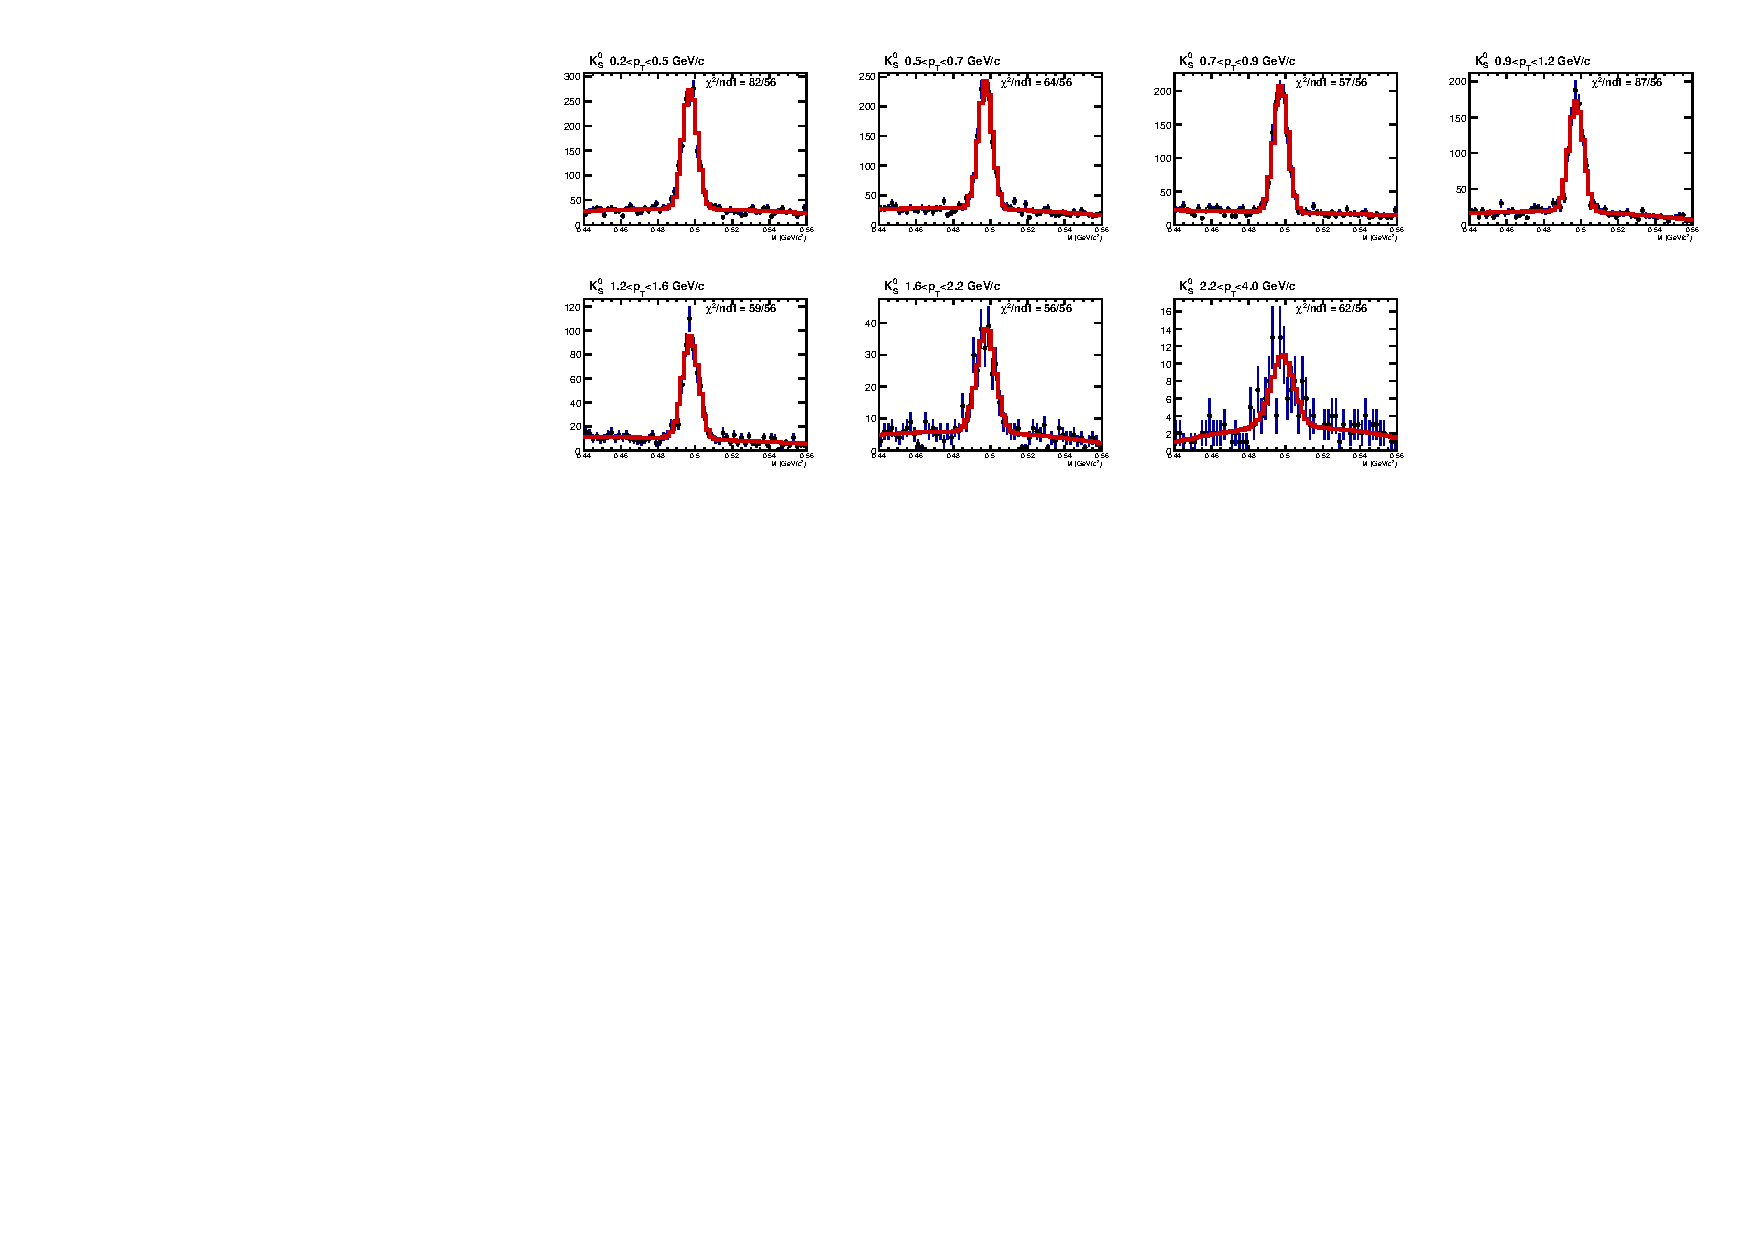
\includegraphics[width=\textwidth]{fig_mass_Ks_A_kappa}
\caption{\Ks{} mass per V0-\pt{} bin, period A, with $\kappa$ (points), and $N\times$DDSim template + quadratic background at the
\Ks{} best point (red); per-panel Baker--Cousins $\chi^2$/ndf.}
\label{fig:massksA}
\end{figure}

\begin{figure}[H]
\centering
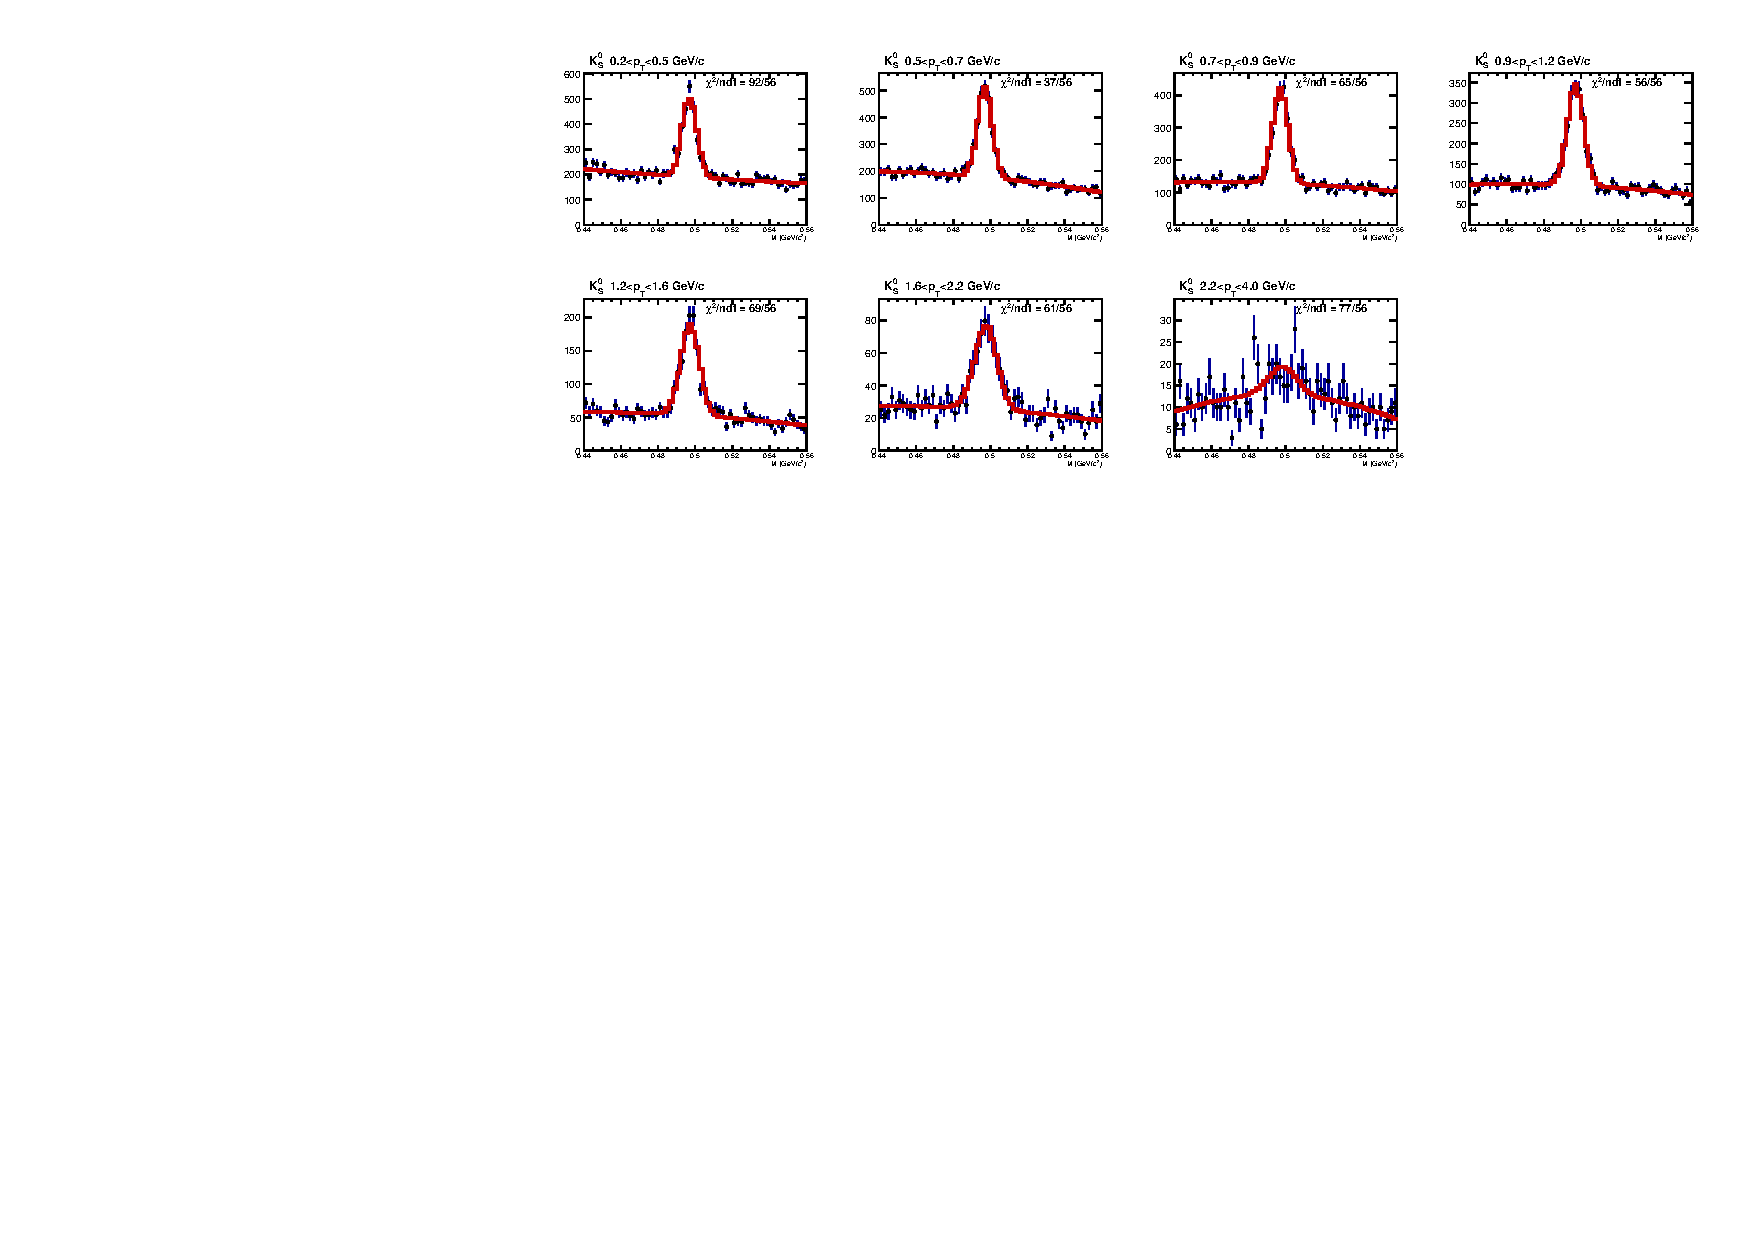
\includegraphics[width=\textwidth]{fig_mass_Ks_B_kappa}
\caption{As Fig.~\ref{fig:massksA}, period B.}
\label{fig:massksB}
\end{figure}

\begin{figure}[H]
\centering
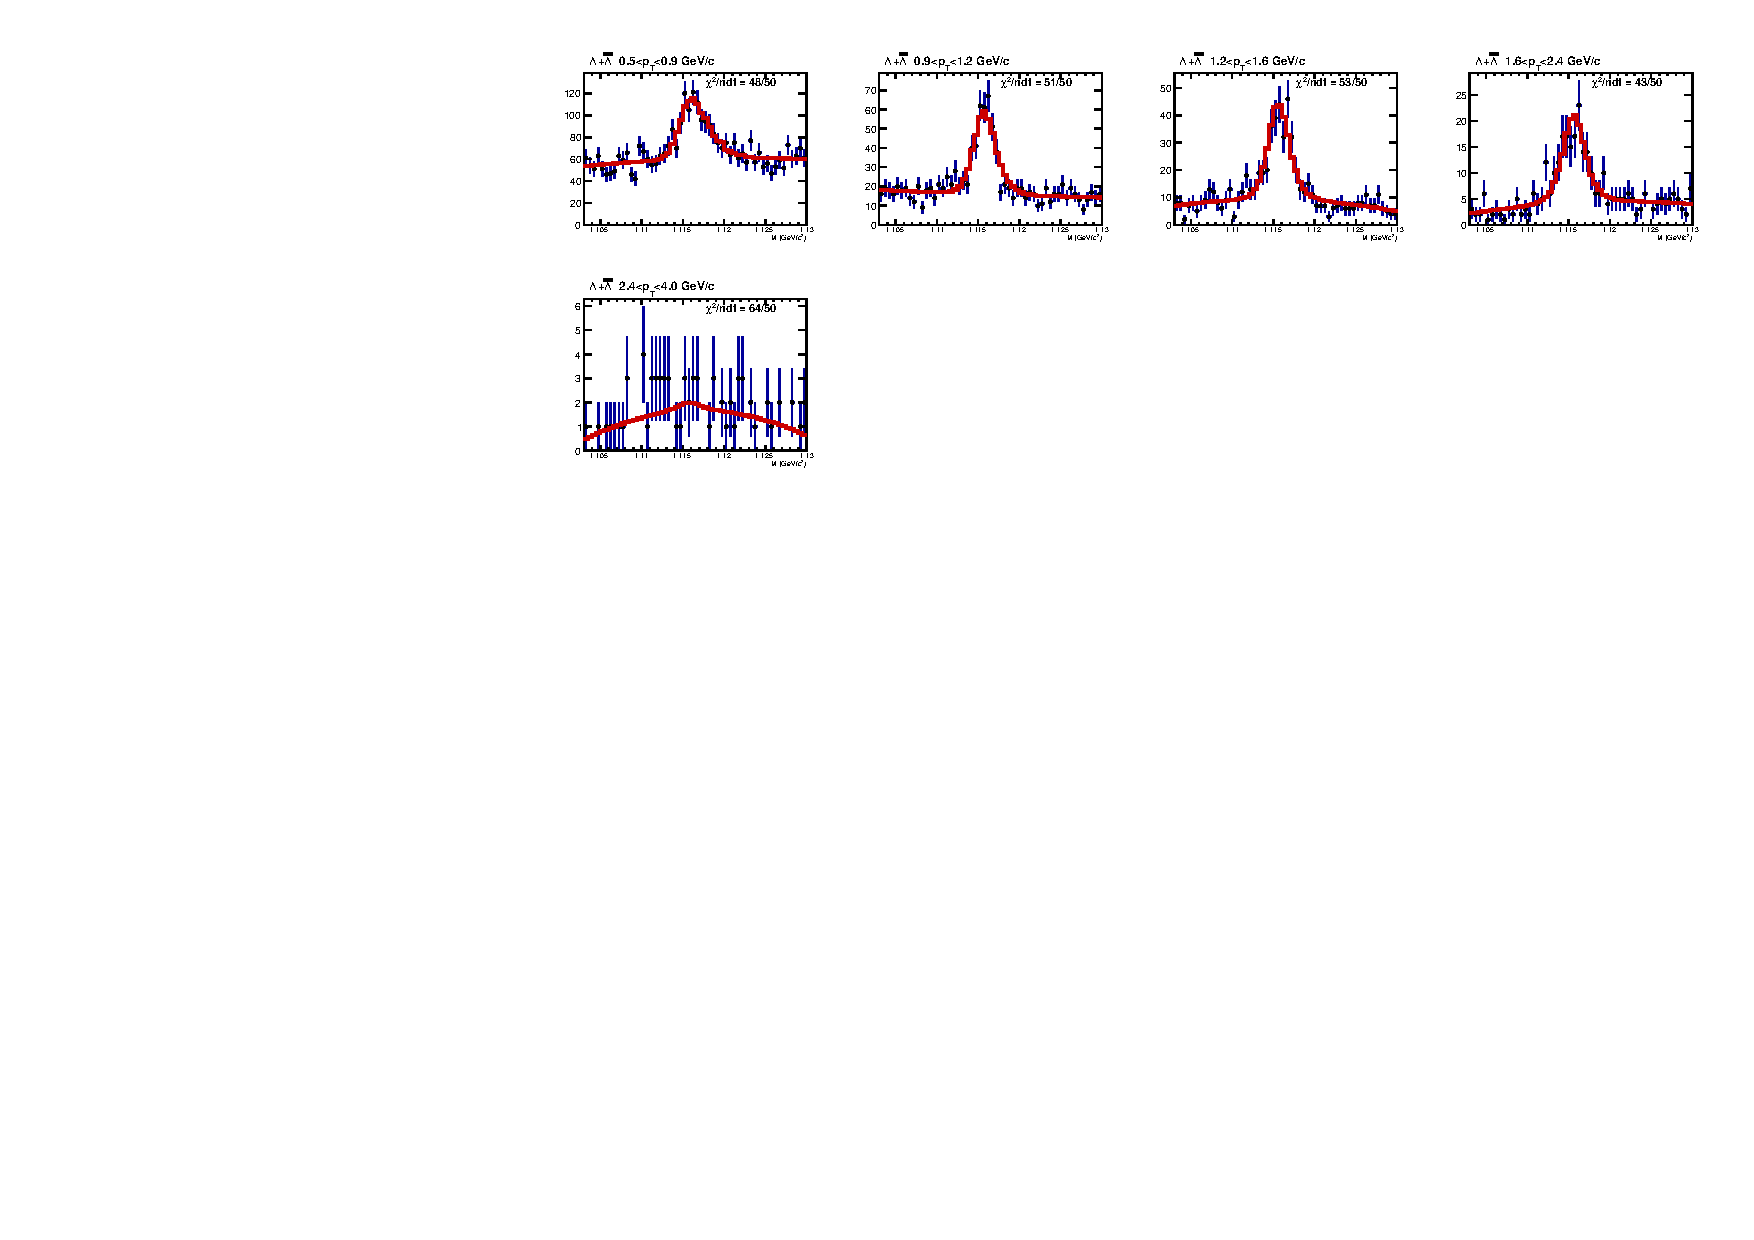
\includegraphics[width=\textwidth]{fig_mass_Lambda_A_kappa}
\caption{\La+$\bar\Lambda$ mass, period A, with $\kappa$; template at the \Ks{} best point (prediction).}
\label{fig:masslaA}
\end{figure}

\begin{figure}[H]
\centering
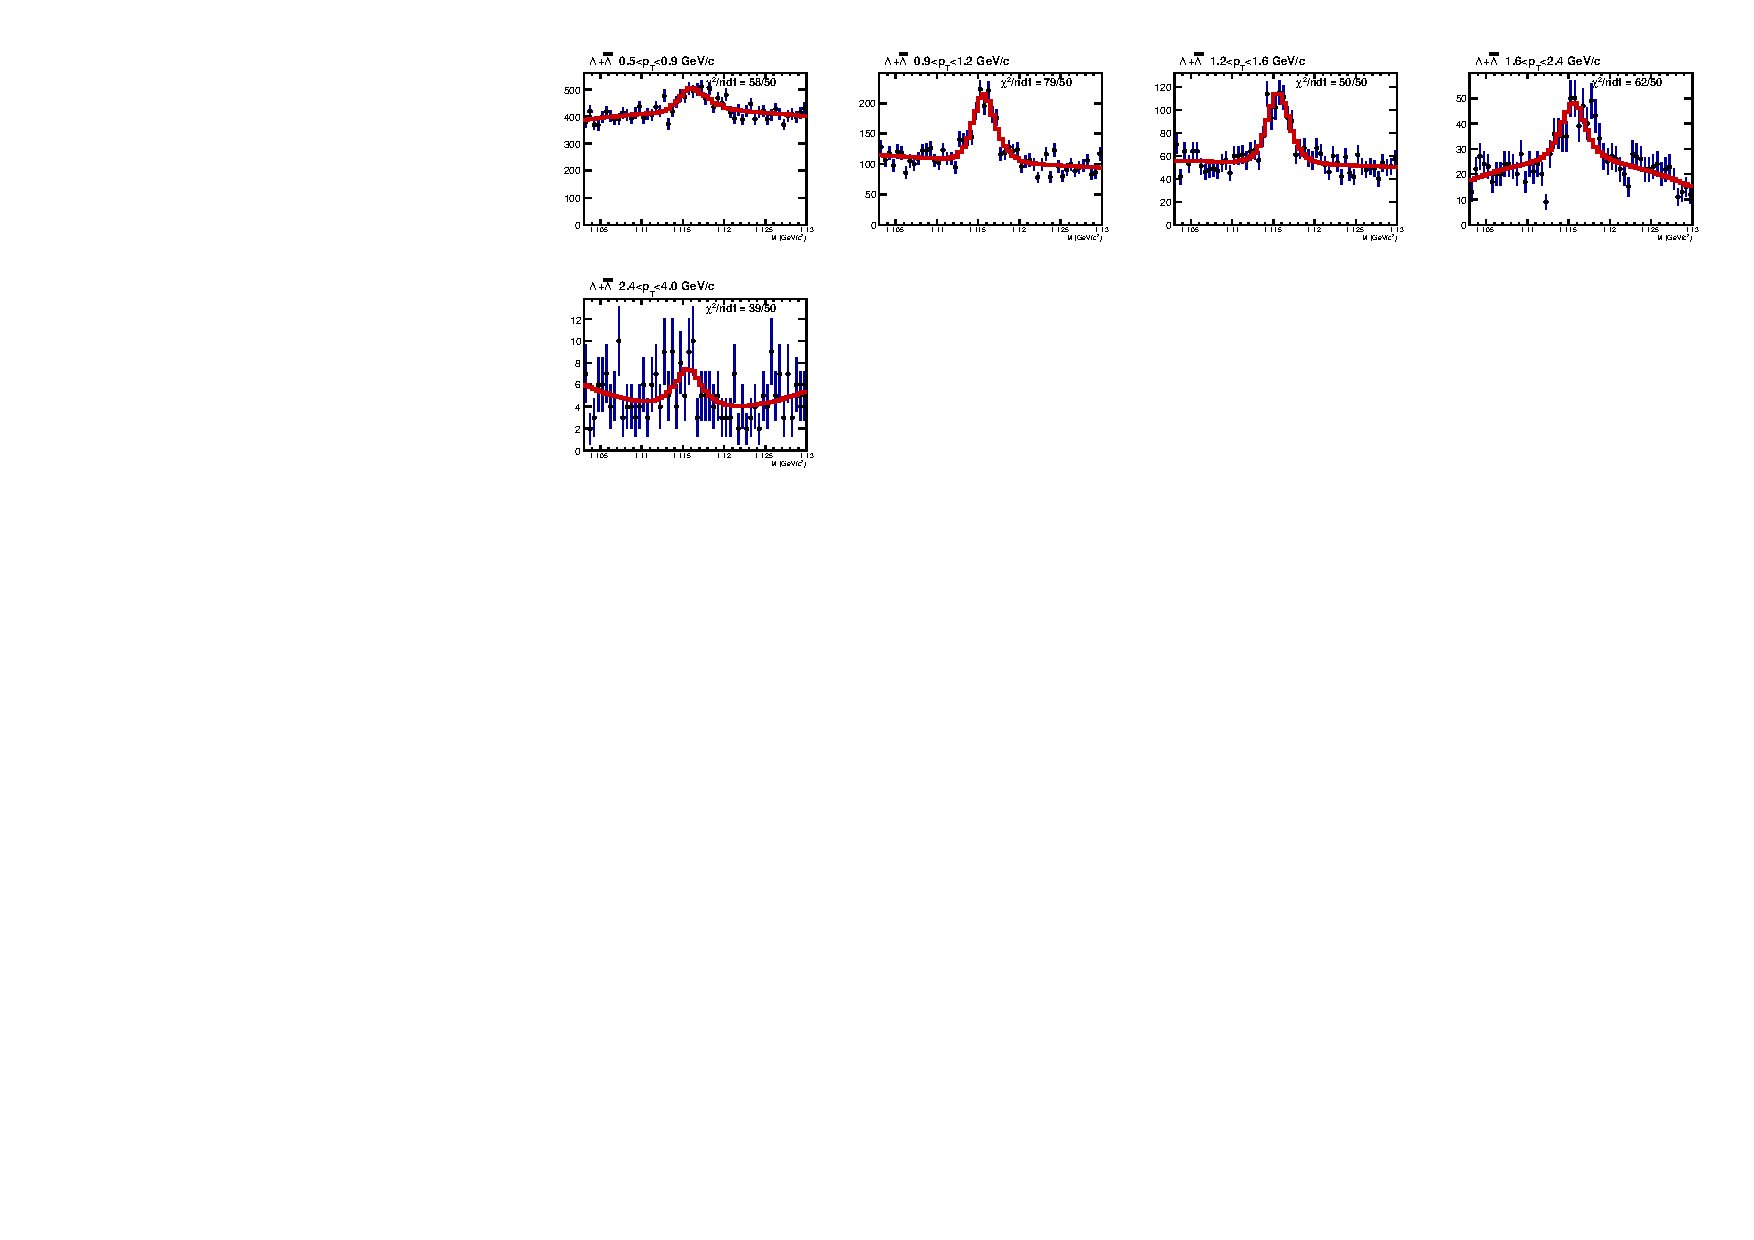
\includegraphics[width=\textwidth]{fig_mass_Lambda_B_kappa}
\caption{As Fig.~\ref{fig:masslaA}, period B.}
\label{fig:masslaB}
\end{figure}

\begin{table}[H]
\centering\small
\caption{Per-bin Baker--Cousins $\chi^2$/ndf of the template fit at the \Ks{} best point of each fit, without and with $\kappa$.}
\label{tab:binchi}
\begin{tabular}{lllcc}
\toprule
period & & V0 \pt{} (GeV/$c$) & no $\kappa$ & with $\kappa$ \\
\midrule
% generated by scripts/make_numbers.py
A & \Ks & 0.2--0.5 & 45.3/56 & 82.2/56 \\
A & \Ks & 0.5--0.7 & 62.4/56 & 64.1/56 \\
A & \Ks & 0.7--0.9 & 59.8/56 & 57.4/56 \\
A & \Ks & 0.9--1.2 & 53.4/56 & 87.3/56 \\
A & \Ks & 1.2--1.6 & 80.6/56 & 59.5/56 \\
A & \Ks & 1.6--2.2 & 79.0/56 & 56.3/56 \\
A & \Ks & 2.2--4.0 & 84.1/56 & 61.6/56 \\
A & \La & 0.5--0.9 & 55.0/50 & 47.9/50 \\
A & \La & 0.9--1.2 & 53.6/50 & 50.7/50 \\
A & \La & 1.2--1.6 & 54.2/50 & 53.0/50 \\
A & \La & 1.6--2.4 & 70.5/50 & 43.4/50 \\
A & \La & 2.4--4.0 & 63.2/50 & 63.7/50 \\
\midrule
B & \Ks & 0.2--0.5 & 75.9/56 & 91.9/56 \\
B & \Ks & 0.5--0.7 & 58.6/56 & 36.8/56 \\
B & \Ks & 0.7--0.9 & 57.0/56 & 65.4/56 \\
B & \Ks & 0.9--1.2 & 66.7/56 & 56.4/56 \\
B & \Ks & 1.2--1.6 & 58.2/56 & 69.1/56 \\
B & \Ks & 1.6--2.2 & 96.4/56 & 61.1/56 \\
B & \Ks & 2.2--4.0 & 60.4/56 & 76.7/56 \\
B & \La & 0.5--0.9 & 52.1/50 & 58.0/50 \\
B & \La & 0.9--1.2 & 80.2/50 & 78.7/50 \\
B & \La & 1.2--1.6 & 60.7/50 & 50.3/50 \\
B & \La & 1.6--2.4 & 67.6/50 & 62.4/50 \\
B & \La & 2.4--4.0 & 57.9/50 & 39.4/50 \\

\bottomrule
\end{tabular}
\end{table}
